jul% Acá se define el tamaño de letra principal:
%
\documentclass[11pt]{article}
\usepackage{subfig}
\usepackage{amsfonts} 

%
% Título y autor(es):
%
\title{Practical}
\author{Massaro\\ Soraruf}

%------------------------- Carga de paquetes ---------------------------

% Definición del tamaño de página y los márgenes:
%
\usepackage[a4paper,headheight=16pt,scale={0.7,0.8},hoffset=0.5cm]{geometry}

%
% Vamos a escribir en castellano:
\usepackage[english]{babel}
\usepackage[utf8]{inputenc}
\usepackage{tabularx}
\usepackage{booktabs}

%\usepackage{helvet}
%\renewcommand\familydefault{\sfdefault}
\usepackage{amsmath,amssymb}
\usepackage{accents}
\usepackage{amsmath}
\usepackage{comment}
\usepackage{algorithm}
\usepackage{algpseudocode}
\usepackage{hyperref}
\usepackage[hidelinks]{hyperref}
\usepackage{algorithm}
\usepackage[noend]{algpseudocode}
\numberwithin{equation}{section}
\numberwithin{figure}{section}
\numberwithin{table}{section}

\usepackage{fancyhdr} %Cabecera y pie de página     

%
% Para poner el texto "Figura X" en negrita:
% (Si no tenés el paquete 'caption2', probá con 'caption').
%
\usepackage[hang,bf]{caption}
% Para poder usar subfiguras: (al estilo Figura 2.3(b) )
%
% Para poder agregar notas al pie en tablas:
%
%\usepackage{threeparttable}

\DeclareMathOperator{\E}{\mathbb{E}}

%------------------------------ graphicx ----------------------------------

\usepackage[pdftex]{graphicx}
\pdfcompresslevel=9

%
% Todas las imágenes están en el directorio tp-img:
%
\newcommand{\imgdir}{includes}
\graphicspath{{\imgdir/}}

\renewcommand{\baselinestretch}{1.1}   %Interlineado

%------------------------- Inicio del documento ---------------------------

\begin{document}

%
% Hago que en la cabecera de página se muestre a la derecha la sección,
% y en el pie, en número de página a la derecha:
%
\pagestyle{fancy}
\renewcommand{\sectionmark}[1]{\markboth{}{\thesection\ \ #1}}
\lhead{}
\chead{}
\rhead{\rightmark}
\lfoot{}
\cfoot{}
\rfoot{\thepage}

%
% Carátula:
%
\begin{titlepage}

\thispagestyle{empty}

\begin{center}
\includegraphics[scale=0.5]{Includes/0-siegel.eps}\\
\large{\textsc{Ludwig-Maximilians-Universität München}}\\
\large{MSc Data Science }\\
{\textsc{Master Thesis}} \\ 
\vspace{0.5cm}
\small{Summer Semester 23 }
\end{center}

\vspace{2cm}

\begin{center}
\Large{\textsc{ Multi-Image Super Resolution and Domain Adaptation Techniques applied to Thermal Remote Sensing}} \\
June 30, 2023
\end{center}

\vspace{2cm}

\begin{tabbing}
	Student:\hspace{-1cm}\=\+\hspace{1cm}\=\hspace{6cm}\=\\
		Massaro, Patricio	\>\> \\
			\>\footnotesize{$<$p.massaro@campus.lmu.de$>$}\\
		\\
\end{tabbing}

\vfill

\hrule
\vspace{0.2cm}
\noindent\small{Master Thesis\hfill }
\end{titlepage}

\input{sections/Acknowledgement.tex}

\tableofcontents
\newpage

%
% Inicio del TP:
%
\setcounter{page}{1}


\section{Introduction} \label{sec:intro}

This thesis delves into the intricate realm of MISR and Domain Adaptation techniques, tailored for the domain of thermal remote sensing, with an emphasis on the challenges and innovations within the unpaired dataset context. Thermal imagery, with its unique sensitivity to temperature variations, offers an invaluable perspective for phenomena such as wildfire tracking and climate change studies. However, the native resolution of such thermal images often falls short of the detail necessary for fine-grained analysis, propelling the need for advanced SR methods.

    \subsection{Storyline}

    \begin{itemize}
        \item Forest fires are dynamic events that change quickly over time. They could be monitored using remote sensing LWIR -> LST
        \item Spatio-temporal trade off: Big missions have high resolution but bad revisit frequency. This is where forest plays a role. But can we improve the resolution using post-processing techniques?
        \item Super resolution is an ill-posed problem, supervised deep learning techniques are generally used in the current literature.
        \item MISR leverages on subpixel differences present in several images taken from the same scene, potentially giving more information to generate an SR image. The potential increase in performance comes with the cost a data-processing overhead.
        \item One of the biggest challenges in super resolution is to create proper datasets for model training. Usually the degradation model used to generate HR-LR pairs is very simplistic compared to real cases. This problem is called domain gap.
        
        \item To bridge the gap, techniques like domain adaptation using gans could be used to estimate the degradation process and generate more realistic datasets, that will translate in better production-ready models.
        \end{itemize}

    \textbf{This thesis covers three main questions:}

    \begin{itemize}
        \item How does the performance of Multi-Image Super Resolution (MISR) compare to Single-Image Super Resolution (SISR), considering the pre-processing burden associated with MISR?

        \item How do traditional baseline degradation models, such as gaussian blurring, compare against a probabilistic model that aligns the distribution of a source domain (e.g., ECOSTRESS) to our  target domain (FOREST-2)?

        \item What impact do the different degradation models have during the inference stage, when the SR models are used in real data.
    \end{itemize}
         
          
        



    

    \newpage

    \subsection{Wildfire monitoring using thermal remote sensing}

    

    \subsubsection{Spatio-temporal trade-off}

\section{Super resolution} \label{sec:SR}

    Super resolution refers to an image processing technique looking to recover a corresponding high-resolution image from a low-resolution version of it, with applications that range from natural images \cite{zeyde2010single}, \cite{martin2001database} to satellite \cite{valsesia2021permutation} and medical imaging \cite{bashir2021comprehensive}. SR remains a challenging task in computer vision because it is considered an ill-posed problem: several HR images can generate exactly the same LR image. 

       \begin{figure}[H]
            \centering
            \includegraphics[width=\textwidth]{Includes/2-SR-ill-posed.jpg}
            \caption{Example of super resolution as an ill posed problem. A blurry picture of Barack Obama can be generated from an HR image of another person.}
            \label{fig:2-SR-ill-posed}
        \end{figure}
    
    Super resolution was first proposed in the 1960s, while the first use of multiple images dates of 1989. 
    Traditional interpolation-based methods for upsampling images were the first type of algorithms used for super resolution.
    The most common techniques are nearest-neighbor, bilinear and bicubic interpolation.
    Nearest-neighbor interpolation is the most straightforward algorithm, as the interpolated value is based on its nearest pixel values. 
    While this method requires almost no calculations, the results are usually blocky because there are no interpolated smooth transitions.
    Bilinear and bicubic interpolation produces smoother transitions using linear or cubic interpolation in both axes. 
    Bilinear interpolation needs a receptive fields of 2x2 and is usually faster, bicubic needs a receptive field of 4x4. 
    The latter is the most common baseline to quantify the improvement of any super resolution algorithm. 

    Machine learning was used for the first time in 2000. 
    Deep learning appears as a branch of machine learning, emphasizing the use of multi-layer neural network cascade for feature exctraction and representation. 
    The rise of the technology wave around 2010 changed the way of solving problems in different branches.
    Instead of piecing together individual feature extraction or functional modules to form a system, the focus is now to optimize parameters by global training after the whole system is designed, what is called end-to-end training.

    \begin{figure}[H]
        \centering
        \includegraphics[width=\textwidth]{Includes/2-end-to-end-training.pdf}
        \caption{In traditional machine learning, the feature extraction step is crucial for performance, requiring a lot of domain knowledge. In deep learning, the feature extraction is learned from the data.}
        \label{fig:2-end-to-end-training}
    \end{figure}

    Super resolution using machine or deep learning is a supervised problem, meaning that the super resolved output must be compared to a HR ground truth image. 
    The difference between the two images is used to calculate the objective loss function that the model seeks to minimize.
    In very few occassions, paired LR-HR images are available.For that reason, the most common approach is to generate the LR images from the HR ground truth using a known degradation model, such as bicubic downsampling + white noise. An example of this method is depicted in Fig. \ref{fig:3-super-resolution-data}. 
    The real degradation process is unknown, and is affected by numerous factors such as sensor-induces noise, lossy compresion, speckle noise, motion blur and optical limitations, between others.
    The disadvantages of using such a simplified degradation process to generate a dataset will be further discussed throughout this work.

    \begin{figure}[H]
        \centering
        \includegraphics[width=\textwidth]{Includes/3-super-resolution-data.png}
        \caption{Example of generating a super resolution dataset, using a simplified known degradation model. Source: \cite{bashir2021comprehensive}.}
        \label{fig:3-super-resolution-data}
    \end{figure}

    

    \subsection{Single-Image Super Resolution}

        In a typical single-image super resolution (SISR) framework, the LR image $I^{LR}$ is modeled as follows:
    
        \begin{equation}
            I^{LR} = D(I^{HR},\Theta) = ( I^{HR} \ast k) \downarrow_s + \ n
            \label{eq:2-degradation-equation}
        \end{equation}
    
        Where $\Theta$ are the function parameters, $I^{HR} \ast k$ is the convolution between a blurring kernel $k$ and the unknown  HR image  $I^{HR}$, $\downarrow_s$ is the downsampling operator with scaling factor $s$ and $n$ is a noise term.
        The relationship between the LR and HR images $D$ is known as the degradation model.
        SISR objective is to solve the inverse equation and obtain $I^{HR}$ from $I^{LR}$, estimating $D^{-1}$ in the process. As stated before, this an extremely ill-posed problem as $D^{-1}$ is not injective, meaning there are infinite possibilities of $I^{HR}$ for which the equation condition hold. 

        A variety of deep learning methods were developed over the years to solve the SR problem, all of them are trained using both low and high-resolution images (LR-HR pairs), most of them generated as in Fig. \ref{fig:3-super-resolution-data}. The models can be classified based on the upsampling method chosen and it's location, the deep learning network and the loss used for learning.


        \subsubsection{Upsampling method}

        The upsampling is essential in deep learning-based SR methods. The most important feature of them is that, as opposed to traditional upsampling methods such as interpolation, they may add new information in the process.

        Sub-pixel convolutional layers performs upsampling by generating several additional channels using convolution, and by reshaping these channels, the resolution of the output is upsampled. The layer has a respective wide field that helps learn more contextual information that results in more realistic details, at the cost of possible artifacts. 

        Deconvolution layers do the inverse of the convolution operation. 
        That means predicting the probable HR image based on the feature maps from the LR image. The process consists on inserting zeros between the pixels of the LR image, and then applying a convolution operation. The amount of zeros is determined by the scaling factor. This method is widely used in SR methods due to its compatibility with the normal convolution, but may cause uneven overlapping in the generated HR image, resulting in a non-realistic image with decreased performance.


        The location of the upsampling layer plays an important role in the architecture. Pre-upsampling SR methods first upsample the LR image and then apply the convolutional layers. The convolutional network task is then to refine the already upsampled image. The biggest drawback is that the dimensions of the image is increzed at the beggining, resulting in higher computational and memory cost than other methods.
        Post-upsampling SR methods first apply the convolutional layers and then upsample the image. The convolutional network task is then to exctract features in a low-dimensional space. The computational cost is lower than pre-upsampling methods, but the extraction of the low level features for a good reconstruction may be more difficult than refining an already upsampled image. 
        This frameworks may be combined by iteratively up and downsampling the image \cite{timofte2015seven}, or by performing progressive upsampling until the desired dimensions are reached \cite{lai2017deep}.

        \subsubsection{Network design}

        In the last years, several deep learning network designs have been proposed to solve the SR problem.  The ones that are most interesting for this work due to their wide use in the literature are residual learning and attention-based learning. 
        
        Residual learning aims to mitigate the vanishing gradient problem that commonly occurs in deep neural network. This is done by adding a skip connection between the input and the output of the network that usually consists in convolutional, batch normalization and non-linear activation layers. This allows the learning of the difference between the input and the output. Mathematically, the residual learning can be formulated as follows:
        \begin{equation}
            F(x) = H(x) - x
            \label{eq:2-residual-learning}
        \end{equation}
        Where $H(x)$ is the mapping function of the network and $x$ is the input. If the residual is local, the skip connection is made over a small block of layers. Global residual makes the input and the output of the whole network to be correlated, which is a very desirable property in SR, as the HR image should have significant correlation with the LR image. In this case, the network transform the LR image into an HR image by generating the missing high-frequency details. 
        Attention learning is the idea where certain factors are given more preference. 

        In channel attention, a particular block is added in the model where global average pooling (GAP) squeezes the input channels; these constants are processed by two fully connected layers to generate channel-wise residuals that define how important is one pixel for each other.
        In SR, most of the models use local fields for the generation of SR pixels, while in a few cases, some textures or patches which are far apart are necessary for generating accurate local patches. This drives the development of attention blocks that extract non-local representations to add information of pixels that are far away from each other.


        \subsubsection{Loss functions}

        As in any supervised learning problem, the selection of the loss function is critical. In SR, they are used for measuring the error in the reconstruction of the HR image. 
        
        Initial research employed the loss at the fundamental block of an image, the pixel.
        The most common loss function is the Mean Squared Error (MSE), which is the average of the squared differences between the predicted and the ground truth images.
        The MSE is the most common loss function in image processing, but it is not the best choice for SR.
        This is because the MSE is very sensitive to outliers and tends to generate overly smooth results, as it converges to the mean of the distribution. Thus, researchers often have used L1 or MAE loss.
        These pixel losses focus on reconstruction fidelity and do not cater for the perceptual quality or textures of the image, resulting in less high-frequency details and overly smooth results. Other were designed to overcome this problem and will be discussed.

        If The perceptual quality is an important objective of the SR task, the differences between the generated and groud truth images could be assessed using an image classification network. The distance between the high-level data representation on a determined layer of the network for both images can be calculated in the following way:

        \begin{equation}
            \mathcal{L}(I^{\text{HR}}, I^{\text{SR}}; N) = \frac{1}{H*W*C}\sum_{i,j,k}(r^{l}_{i,j,k}(I^{\text{HR}}) - r^{l}_{i,j,k}(I^{\text{SR}}))^2
        \end{equation}

        Where $r^{l}$ is the output of the $k$-th channel of the $l$-th layer of the pre-trained classification network $N$ when the input is $I^{HR}$ or $I^{SR}$. $H$, $W$ and $C$ are the dimensions of the layer output (height, width and channels). 
        Commonly used classification networks are VGG \cite{simonyan2015deep} or ResNet \cite{he2015deep}.
        The purpose of the content los is to compare the information about image features from the network. This ensures the visual similarity between the original and generated image by comparing content and not individual pixels. Thus, content loss functions helps producing visually perceptible and more realistic loooking images and are widely used in SR \cite{ledig2017photorealistic,wang2018recovering}. On the other hand, this type of loss may not focus on the physical consistency of the image, resulting in possible artifacts that may look realistic but are non-existant. This is one of the main reasons why the content loss is not used in remote sensing applications.

        The adversarial loss is based on the generative adversarial network (GAN) \cite{goodfellow2014generative}. The GAN is composed of two networks, a generator and a discriminator. The generator is trained to generate SR images that are indistinguishable from the real HR images, while the discriminator is trained to distinguish between the generated and real images. 
        Training is performed in sequencial steps, where the generator is adjusted for better results that may fool the discriminator, and then the discriminator is adjusted to better distinguish between the generated and real images.
        When the generator is able to create outputs that conform to the distribution of the actual data, the discriminator is no longer able to distinguish between the generated and real images. In many cases, the mean squared error is used due to improved results: 

        \begin{equation}
            \begin{aligned}
            \mathcal{L}_{GANg}(I^{SR};D) &= (D(I^{SR}) - 1)^2 \\ 
            \mathcal{L}_{GANd}(I^{HR}, I^{SR};D) &= (D(I^{SR}))^2 + (D(I^{HR}) - 1)^2
            \end{aligned}
        \end{equation}

        Where $D$ is the discriminator network. 
        Results show that although the adversarial loss yielded lower physical consistency metrics, content and perceptual metrics were improved. 
        The use of the discriminator was able to regenerate intrincate patterns that were very difficult to learn using ordinary deep learning methods. 
        This is because the pixel-loss-based solutions perform a pixel-wise aggregation of the posible solutions in the pixel space, while adversarial loss drives the reconstruction towards the natural image manifold, producing more perceptually convincing solutions. 
        The main drawbacks of the adversarial loss are the inherent instability in the training of GANs and the probable degradation in physical consistency metrics.
        The latter is the main reason why this type of loss will not be used throughout this work.

        \begin{figure}[H]
            \centering
            \includegraphics[width=\textwidth]{Includes/2-gans-natural-manifold.png}
            \caption{Illustration of patches from the natural image manifold and results coming from MSE pixel-loss (red) and GANs (orange). source:\cite{ledig2017photorealistic}}
            \label{fig:2-gans-natural-manifold}
        \end{figure}

















       




    \subsection{Multi-Image Super Resolution}

        Multi-Image Super-Resolution (MISR) is the task of yielding HR images by fusing multiple LR observations of the same scene, which allows the achievement of higher reconstruction accuracy than relying on only one image.
        The development of this approach progressed at a slower pace due to the extesive pre-processing requirements imposed on the input, as this algorithms have a high sensibility to the input variability and their proper co-registration.  

        When the input images are of the same nature, but taken at different points in the temporal dimension, the problem is often called multi-image super resolution.
        On the other hand, when the images are taken at the same time but they come from different sensors and show different spectral bands, it is called multi-spectral super resolution, which will be further discussed. 

        The main problem in MISR is the difficulty to generate a dataset with multiple images of the same scene, and it is the main reason why SISR is more popular.
        In 2019, the European Space Agency (ESA) organized an SR challenge  \cite{martens2019superresolution} based on real-world scenes acquired by the PROBA-V satellite, each of which contains an HR image (100m GSD) coupled with at least nine LR images that are not perfectly co-registered and they may be taken months apart. 
        This challenge, with a not-synthetically generated HR-LR image pairs, fostered a new generation of model architectures that are able to fuse the multiple LR images to create better reconstructions \cite{Salvetti_2020,Bordone_Molini_2020}.
         Both of the cited networks were tested in synthetically generated datasets throuhout this work and showed better performance than SISR networks, but they were discarded because of the impossibility to have a multi-image dataset using real FOREST-2 images.

        \begin{figure}[H]
            \centering
            \includegraphics[width=\textwidth]{Includes/2-MISR.jpeg}
            \caption{Multi-image super resolution algorithms combine multiple low-resolution image acquisitions into a high-resolution image. Source: \cite{MISR2007}}
            \label{fig:2-MISR}
        \end{figure}
        
        \subsubsection{Multi-spectral super resolution}

        Also Referred to as "hyper-spectral super resolution" in the literature, The term "Multi-Spectral" emphasizes the use of multiple spectral bands, in contrast with the multi-image approach detailed previously. While the concept bears similarities to MISR, the key distinction lies in MSSR's use of a single scene captured with different spectral bands, as opposed to multiple images, to reconstruct a superior, super-resolved image.

        In the context of MSSR, each spectral band, corresponding to a specific wavelenght range, provides unique information about the observed scene. Some of the spectral bands yield better resolution because of their physical properties and the costs related to their sensors. Using this higher resolution bands to increase the detail in the lower bands seems like a resaonable approach.

        Traditional pan-sharpening algorithms could be considered as deterministic MSSR  algorithms. They are usually used to increase the resolution of a multi-spectral RGB image using the panchromatic band. The overlap between the wavelengths of the bands makes this algorithm straightforward and useful. However, it is ill-suited for Thermal Infrared (TIR) data due to the disjointed spectral domains of the visible and TIR bands.
        The result of pansharpening TIR data is shown in Fig. \ref{fig:2-pansharpening}  While the general resolution of the image is improved, several TIR hotspots are darkened and highlights from the visible bands are translated to the super-resolved image. This is particularly problematic for clouds, which have an inverse spectral response in the TIR and RGB bands. 
        
        \begin{figure}[H]
            \centering
            \includegraphics[width=\textwidth]{Includes/2-pansharpen.png}
            \caption{Example of Pan-sharpening on TIR data using a panchromatic band. (a) Panchromatic band, (b) HR TIR image, (c) Downsampled version of the TIR image , (d) Pansharpened image. 
            The pan-sharpened image is less blurry than the LR, but a lot of artifacts are produced, specially in clouds. Source: \cite{myself2023}}
            \label{fig:2-pansharpening}
        \end{figure}

        In \cite{myself2023}, A deep learning MSSR network is trained assuming the presence of common information between low-resolution LWIR images and their higher resolution RGB counterparts, with the objective of creating a super-resolved product in the LWIR band by an effective fusion. This improved image retains the essential thermal information, while simultaneously incorporates enhanced spatial resolution details captured from the visible bands. 
        MSSR remains a more promising alternative than MISR because it doesn't have the pre-processing burden that the latter has, as the images are well co-registered in the spatial and temporal domain.
        Additionally, most satellites have multi-spectral sensors, making the dataset generation much easier.

    \subsection{The domain gap problem} \label{subsec:domaingap}
 
        SR is a supervised problem, the super resolved image is compared to the HR ground truth and the differences (pixel-by-pixel or perceptual) drive the gradients of the neural network to minimize the loss, in a fully supervised manner. 
        The objective of this work is to increase the resolution of FOREST-2 images, but a high resolution version of FOREST-2 is not available. 
        The only alternative is to use scenes from other missions that have a higher resolution.

        Most of the research in the field of SR is conducted by artificially producing HR-LR pairs by downscaling the HR images with known kernels, as in Fig. \ref{fig:3-super-resolution-data}.
        However, this is rarely the case when using "non-ideal", real world images.
        In spite of their success on synthetic datasets, the poor generalization capacity of the trained SR networks limits their application in real scenarios, leading to blurry images and strange artifacts in the SR results \cite{lugmayr2020ntire}.

        The domain gap problem occurs when there are systematic discrepancies between data use for training and the real-world data. 
        This is described in Fig. \ref{fig:2-domain-gap}, where the HR image is processed through different known degradations. 
        If an SR model is trained using the left-most degradation, it will produce undesirable results if LR images generated by the other degradations are used as input.
        In this example, the left-most degradation seems to have better resolution and less noise than the rest. This will lead to noisier and blurrier results when using the other degradations as input.

        \begin{figure}[H]
            \centering
            \includegraphics[scale=0.4]{Includes/2-domain-gap.pdf}
            \caption{Effects of different degradation models on one HR image. Source: \cite{liu2021blind}}
            \label{fig:2-domain-gap}
        \end{figure}

    \subsection{Blind image Super Resolution}

        The problem of SR with an unknown degradation process is known as blind SR. 
        Growing attention has been paid to blind SR in recent years, towards filling the domain gap presented in \ref{subsec:domaingap}.
        A schematic diagram of the problem is shown in Fig. \ref{fig:2-DomainGap}. 
        Non-blind SR methods assume that the degradation process is known, and maps the bicubic downsampled LR image to the natural HR image space.
        However, an arbitrary LR input image, as a scene captured by a satellite, is usually degraded by an unknown process, which is difficult to be modelled explicitly.
        The arbitrary LR input is not in the same domain as the bicubic downsamopled LR image, and thus the non-blind SR methods are not successful in the super resolution process.
        There will be a large domain gap between the SR output and the desired image samples from the target natural HR domain, leading to a poor-quality result.
        Blind SR methods, on the other hand, aim to learn the degradation process from the training data, and map the arbitrary LR input image to the natural HR image space.
        
        \begin{figure}[H]
            \centering
            \includegraphics[width=\textwidth]{Includes/2-DomainGap.png}
            \caption{Domain interpretation of differences between non-blind and blind SR. Source: \cite{liu2021blind}}
            \label{fig:2-DomainGap}
        \end{figure}

        In the literature, two main approaches exist to bridge the gap: 
        Explicit modelling based on an extension of eq. \ref{eq:2-degradation-equation} and implicit modelling thought distribution learning of the degradation process.
        Explicit modelling can be further classified into two sub-categories according to whether they employ external datasets or rely on a single input image to solve the SR problem.


        \subsubsection{Explicit modelling with external dataset}

        This kind of methods use an external dataset to train an SR model well adapted to  variant blurring kernels and noises. 
        Typically, a traditional SISR is employed and an estimation of the kernel and the noise is used as a conditional input along with the LR image.
        After the training process, the model will be able to produce good results only in the now bigger pool of degradation types covered in the training dataset.
        According to whether the degradation is estimated or given, this approach can be further classified into two sub-categories.


        Explicit modelling without kernel estimation aims to directly concatenate a pre-defined degradation map to the LR input, as depicted in Fig \ref{fig:2-external-dataset-stretching}. 
        This allows feature adaptation according to the specific degradation model and helps to cover multiple degradation types during training. 
        The PCA technique used to project the degradation map can be replaced with a shallow neural network that may learn a kernel mapping that better fits the specific SR model used.

        \begin{figure}[H]
            \centering
            \includegraphics[width=\textwidth]{Includes/2-external-dataset-stretching.png}
            \caption{Dimensionality stretching strategy to concatenate the degradation map to the LR input. 
                     The vectorized kernel is projected onto a space of a lower dimensionality, and then stretched to generate $t$ feature maps with the same shape of the input image.
                     The noise level is also concatenated. Source: \cite{zhang2018residual} }    
            \label{fig:2-external-dataset-stretching}
        \end{figure}

        The biggest drawback  of this approach is that it relies on an additional input of degradation estimation, specially the kernel. 
        Howerver, estimating the correct kernel from an arbitrary LR image is not easy and kernel mismatch will result in a dramatic loss in SR performance.
        This method remains feasible only when a way of obtaining a reliable degradation estimation is available.
        Otherwise, a manual process to find the best input for better result is needed.
        
        Explicit modelling with kernel estimation aims to estimate the kernel from the LR input image in an iterative way until a good enough result is obtained \cite{gu2019blind}.
        The main idea is to take advantage of intermediate SR results because some of the artifacts caused by kernel mismatch show regular patterns that a corrector network can use to perfrom kernel correction.
        Methods like \cite{luo2020unfolding}, enhance the approach by unifying the kernel correction and SR network into an end-to-end trainable network. 
        However, the iterative nature of this method leads to higher inference time. Additionally, the optimal number of iterations is not known and must be determined empirically.

        Other approaches propose to learn a bling SR model by merely covering more degradations with more realistic kernels in the training dataset, creating a large pool.
        Kernels from this pool are used to synthetize the training pairs in a non-blind setting. 
        The more general training dataset enables the SR model to adapt to real input images. 
        However, it is very hard to cover all the possible degradation types in the real world, and the model will fail when facing a new degradation type.


        \subsubsection{Explicit modelling with single image}

        SR modelling with a single image is based on internal statistics of natural images: patches of a single image tend to recur within and across different scales of the image \cite{zontak2011}.
        This characteristic is very powerful, since it is image-specific and unsupervised. It was used first in 2009 in a method that does not used deep learning \cite{glasner2009}, and gained traction with KernelGAN \cite{bellkligler2020blind}. 
        KernelGAN interprets the maximization of patch recurrence as a data distribution learning problem, assuming that the downsampled version of an LR image generated by the optimal kernel should share the same patch distribution with the original LR input.
        Using a GAN framework, a deep linear network is used as a generator to parametrize the underlying SR kernel, and a discriminator distinguishes generated patches from those of the original LR image.
        Once training finishes, the output of the generator is an estimation of the blurring kernel of the input image. 

        \begin{figure}[H]
            \centering
            \includegraphics[width=\textwidth]{Includes/2-kernelGAN.png}
            \caption{KernelGAN schematic diagram. The discriminator tries to distinguish between the generated patches and the original LR image patches. G learns perform 2x downscaling while fooling the discriminator by maintaining the same distribution of patches. Source \cite{bellkligler2020blind}}    
            \label{fig:2-kernelGAN}
        \end{figure}

        This idea of self-supervision based on patch recurrence is also applied to perform SR without pre-training, as in zero-shot super resolution (ZSSR) \cite{shocher2017zeroshot}.
        In this case, the training is conducted using HR-LR pairs generated from a single LR image.
        The original input is regarded as HR and downsampled versions of it as LR using a kernel. 
        The network trained on these image pairs will be capable of inferring relationships across different scales which is then used to super-resolve the input.
        ZSSR is still not fully blind, it requires an estimated blur kernel as input. 
        For that reason, a joint framework that combines ZSSR and KernelGAN yields very good results.
        For a given image, KernelGAN estimates the blurring kernel that is then used in ZSSR to perform super resolution.

        While the idea of self-supervision is very flexible and efficient, its basic assumption may fail in certain cases.
        Hence, this approach can only produce favourable SR outputs for a limited set of images that have recurring contents across scales.



        \subsubsection{Implicit modelling} \label{subsubsec:implicit-modelling}

        Implicit modelling aims to grasp the underlying degradation model through learning from an external dataset.
        On paired HR-LR images, the SR model is already enough. However, these datasets are rarely available in real-world scenarios.
        Usually the data available is unpaired, meaning that HR images and LR images with realistic degradations are available, but there is no correspondence between them.
        Existing approaches exploit the data distribution learning ability of GANs, where discriminators are used to distinguish between the generated images from the real ones, pushing the generator towards an appropiate direction.
        
        First attempts for implicit modelling were based on CycleGANs \cite{CycleGAN2017}, that consists of two generators and two discriminators that move from domain A to B and viceversa. 
        The cycle consistency loss is based on the principle that after a round-trip transformation, the original image should be recovered.
        In CinCGAN \cite{yuan2018unsupervised}, the HR input is transformed using bicubic downsampling before doing SR with a pre-trained network and is regarded as the clean LR domain.
        Two CycleGAN structures are applied to transform the LR input to the clean LR domain and to the HR domain. 
        This way, no paired data is necessary.

        Another way of performing implicit modelling is using a single GAN to learn the degradation process from HR to LR, and generate a supervised paired dataset that can be used for training the SR network.
        The generator simulates the degradation from the HR domain to the LR domain and the discriminator distinguishes between the generated LR images and the real LR images.
        In these methods, such as \cite{luo2022learning,bulat2018learn}, usually the discriminator architecture is focused to distinguish the images using the high-frequency contents of them, due to the fact that degradations usually have a big overlap at lower frequencies.
        To further reduce the domain gap, several extensions of the method are proposed. 
        In \cite{wei2020unsupervised}, both the generated and real LR images are used to train the SR model.
        The super resolved version of the generated LR images can be compared with the original HR input using a pixel-wise loss, and the super resolved real LR images can be used for training trough a discriminator that distinguishes between them and the HR images.

        \begin{figure}[H]
            \centering
            \includegraphics[width=\textwidth]{Includes/2-degradation-gan.png}
            \caption{Degradation GAN schematic diagram. The architecture includes one LR generator, on SR network and two discriminators. Source: \cite{bulat2018learn}.}    
            \label{fig:2-degradation-gan}
        \end{figure}
        
    
        While very flexible, limitations of implicit modelling are the dependency on huge dataset that is just not possible in some applications. 
        Additionally, several artifacts may be produced in the SR results due to the difficulty and instability of GANs training.
        The choice of the generator in the case of degradation learning GAN is also very important, if it is not well constrained enough, it will produce unrealistic results that will misguide the SR network and lead to poor results even after long training sessions.
         
         




        
























        
        
        

        

        

        










        

\clearpage
\section{Domain adaptation} \label{sec:domain_adaptation}
    \subsection{GANs for domain adaptation}

    \subsection{Learning the degradation process}

    \subsection{Probabilistic degradation process}


\clearpage
\section{Methodology} \label{sec:methodology}
    
    \subsection{Baseline Degradation model} \label{subsec:baseline_degradation_model}

        Early super-resolution methods commonly generated high-resolution (HR) to low-resolution (LR) samples using predefined degradation techniques, with bicubic downsampling being the most used setting \cite{zhang2018residual}. This kind of synthetic data, while easy to obtain, often results in a domain gap problem, where the data used for training and assessing the model do not come from the same distribution as real data. This gap usually to performance drops when the models implemented in production environments. A possible solution is to synthesize samples with a stochastic degradation model, which includes a set of multiple blurring kernels and several random noises configurations. The larger degradation space grant these models better generalization capabilities and experts be part of the kernel definition process, based on prior knowledge of the degradation process. Unfortunately, the variety of predefined degradation's is still limited and still fail in most applications.

        A degradation model like this one will be used as a baseline for this work.
        

        \subsubsection{Blurring Kernel}

        \begin{figure}[h!]
                \centering
                \includegraphics[width=\linewidth]{Includes/4-degradation_kernels.pdf}
                \caption{Example of kernels used in a stochastic degradation model. (a),(b) and (c) are generated using a symmetric variance on the x and y axis. (d) (e) and (f) are generated using an asymmetric variances, resulting in much more anisotropic kernels.}
                \label{fig:4-degradation_kernels}
            \end{figure}

        \begin{figure}[h!]
                \centering
                \includegraphics[width=\linewidth]{Includes/4-degradation-kernel-examples.pdf}
                \caption{Effects of different blurring kernels on the HR-LR generation. The upper row contains images generated using blurring kernels with symmetric distributions. The lower rows contains images generated using asymmetric distributions for the variances, resulting in highly anisotropic kernels.}
                \label{fig:4-degradation_kernels}
            \end{figure}
            
        \subsubsection{Radiometric error correction}

        As reported by the ECOSTRESS instrument sheet,\cite{ECOSTRESS2023INSTRUMENT} its nominal radiometric accuracy at 300K is 0.5K. FOREST-2 target radiometric accuracy is 1K. This difference in accuracy should be taken into account. To align these accuracies, we first calculate the additional error required using the following equation:

        \begin{equation}
            e_{\text{forest}} = \sqrt{e_{\text{eco}}^2 + e_{\text{extra}}^2} 
            \label{eq:4-radiometric-error-correction}
        \end{equation}
        
        where $e_{\text{eco}}$ is the ECOSTRESS error, and $ e_{\text{extra}}$ is the additional error required for FOREST-2.
        
        Using the above equation, we find that an additional radiometric error of approximately 0.8660K is needed. The next step involves converting this extra error into a radiance value. This requires calculating the derivative of the Planck equation at 300K, which is done numerically as follows:
        
        \begin{equation}
            \frac{\partial B}{\partial T} = \frac{B(\lambda, T + \delta T) - B(\lambda, T)}{\delta T}
            \label{eq:4-planck-derivative}
        \end{equation}  
        
        By multiplying the results of equations \ref{eq:4-radiometric-error-correction} and \ref{eq:4-planck-derivative}, we can obtain the radiance error for both FOREST LWIR bands. The additional radiance errors for LWIR1 and LWIR2 bands are found to be \(1.5472 \times 10^{-1}\) W/sr/m\(^2\)/\(\mu m\) and \(1.1444 \times 10^{-1}\) W/sr/m\(^2\)/\(\mu m\), respectively.

        The difference in radiances will be split into two components. On one side, the cold Bias represents a systematic error in the measurement, this error acknowledges discrepancies that can be attributed to sensor calibration and atmospheric conditions. On the other side, the random noise accounts for unpredictable fluctuations in the measurement process. It could be due to a variety of sources like electronic noise in the sensor, random atmospheric disturbances, or other stochastic factors. As the extent of each component is not known and to give more variability to this basic degradation model, a random factor $\phi \in [0,1] $ is introduced so that:

        \begin{equation}
        \begin{aligned}
            \varepsilon_{\text{final}} &= (1 - \phi) \times \varepsilon_{\text{radiance}} + \phi \times \eta \times \varepsilon_{\text{radiance}} \\
            \eta & \sim \mathcal{N} (0,1)
        \end{aligned}
        \end{equation}    

        The effects of the error correction is shown in Fig. \ref{fig:4-radiometric_noise_example}. As the target radiometric error increases with respect to ECOSTRESS scenes, the loss of information is more noticeable.


        \begin{figure}[h!]
            \centering
            \includegraphics[scale=0.55]{Includes/4-radiometric_noise_example.pdf}
            \caption{Effects of different radiometric error corrections on the HR-LR generation.}
            \label{fig:4-radiometric_noise_example}
        \end{figure}
        
    \subsection{Models Architecture}
    
        \subsubsection{SRResNet}

            Introduced in 2017 \cite{ledig2017photorealistic}, SRResnet leverages on residual networks \cite{he2015deep} that employ skip connections to solve the super resolution task. The architecture is detailed in Fig. \textbf{CITE}. Specifically, 16 residual blocks consisting two convolutional layers, followed by batch-normalization layers and ParametricReLU activation functions. The convolutional layers have 3x3 kernels and 64 feature maps. To increase the resolution of the input image, two trained sub-pixel convolution layers are used.

            As this work focuses on having super resolved images with high physical consistency and not on the perceptual superiority of the images, improvements introduced in the publications like the Generative Adversarial Network (SRGAN)  and the perceptual loss for gradient calculation are not used.
        

            \begin{figure*}[h!]
                \centering
                \includegraphics[width=1\textwidth]{includes/3-srresnet-architecture.pdf}
                \caption{ SRResNet architecture. $X_{LR}$ represents the low resolution input image, $X_{SR}$ the super resolved image, which is then compared to the ground truth $X_{HR}$.}
                \label{fig:generator}
             \end{figure*}

        \subsubsection{RAMS}
        \subsubsection{Probabilistic Degradation Model}

            To avoid the domain gap between synthetic and test images, most previous methods try to adaptively learn the degradation process via a deterministic model.
            However, some degradations in real scenarios are stochastic and cannot be determined by the content of the image.
            These deterministic models may fail to model the random factors and content-independent parts of degradations, which will limit the performance of the following SR models.
            In this paper, we propose a probabilistic degradation model (PDM), which studies the degradation D as a random variable, and learns its distribution by modeling the mapping from a priori random variable z to D.
            Compared with previous deterministic degradation models, PDM could model more diverse degradations and generate HR-LR pairs that may better cover the various degradations of test images, and thus prevent the SR model from over-fitting to specific ones.


            Most previous degradation-learning-based SR methods have a common drawback: their degradation models are deterministic, and each HR image can only be degraded to a certain LR image.
            It implies an assumption: the degradation is completely dependent on the content of the image.
            However, this may not hold in most cases.
            Some degradations are content independent and stochastic, such as random noises or blur caused by random shakes of cameras. 
            These random factors and content-independent parts of degradations could not be well modeled by these deterministic models. 
            A better assumption is that the degradation is subject to a distribution, which may be better modeled by a probabilistic model.
            
            We parameterize the degradation with two random variables, i.e., the blur kernel k and random noise n, by formulating the degradation process as the linear function from Eq. \ref{eq:2-degradation-equation}.
            It can be divided into two linear steps \cite{zhu2020unpaired}: 

            \begin{equation}
                \begin{aligned}
                        I^{\text{LR}}_{\text{clean}} &= (I^{\text{HR}} * k) \downarrow_s \\
                        I^{\text{LR}} &= I^{\text{LR}}_{\text{clean}} + n
                \end{aligned}
            \end{equation}
            
            
            The model is trained in a adversarial framework, and the distribution of the LR image could be automatically learned during the training        
            
            Usually,the two steps are mutually independent, as the blur kernels are mainly dependent on the properties of the camera lens while the noises are mainly related to the properties of sensors. 
            Thus, the distribution of the degradation process can be represented as the product of the distribution of $k$ and $n$, which can be modeled by learning the mapping from a priori random variable $z$ to $k$ and $n$.


            \begin{equation}
                p_{D}(D) = p_{k,n}(k, n) = p_{k}(k)p_{n}(n).
            \end{equation}

            To model the distribution of the blur kernel k, we define a priori random variable $z_k$ which is subject to multi-dimensional normal distribution. 
            Then we use a generative module to learn the mapping from zk to k: 

            \begin{equation}
                k = \text{net}K(z_k), \quad z_k \sim \mathcal{N}(0,1),
            \end{equation}

            The spatially variant blur kernel is considered first. This implies that the blur kernel for each pixel of the image is different. In that case, we have

            \begin{equation}
                z_k \in \mathbb{R}^{f_k \times h \times w}, \quad k \in \mathbb{R}^{(k \times k) \times h \times w},
            \end{equation}

            where $f_k$ is the dimension of the normal distribution $z_k$, $k$ is the size of the blur kernel, $h$ and $w$ are the height and width of the image, respectively.
            Generally, the sizes of the convolutional weights  are set as 3 × 3, which indicates that the learned blur kernels are spatially correlated.
            Otherwise, if the spatial size of all convolutional weights is set as 1 × 1, the blur kernel could be approximated by a spatially invariant one, which is a special case of the spatially variant blur kernel with h = w = 1.
            This approximation simplifies the dimensions of the problem drastically and is an appropiate assumption if the crops used for training the model are small enough.
            A Softmax layer is added at the end of the network to guarantee that all elements of k sum to one.
            
            
            To model the distribution of the noise $n$, a vanilla generative module can also be used:

            \begin{equation}
                k = \text{net}N(z_n), \quad z_n \sim \mathcal{N}(0,1),
            \end{equation}

            \begin{equation}
                z_n \in \mathbb{R}^{f_n \times h \times w}, \quad n \in \mathbb{R}^{h \times w \times c},
            \end{equation}

            Where the height, width and number of channels of the image is noted as $h$, $w$ and $c$ respectively. 
            In this work, $c$ is always set to 1.

            In other methods \cite{plotz2017benchmarking}, the noise is modeled as a combination of shot and read noise. 
            It can be approximated as a heteroscedastic Gaussian distribution, which is dependent on the content of the image.

            \begin{equation}
                n \sim \mathcal{N}(0, \sigma_{\text{read}} + \sigma_{\text{shot}} \cdot I^{\text{LR}}_{\text{clean}}),
            \end{equation}

            This indicates that the noise is also related to the image content and the distribution of $n$ should be expressed as:


            \begin{equation}
                k = \text{net}N(z_n,I^{\text{LR}}_{\text{clean}}), \quad z_n \sim \mathcal{N}(0,1),
            \end{equation}

            \begin{figure}[h!]
                \centering
                \includegraphics[scale=0.38]{Includes/3-probabilistic-degradation-model.png}
                \caption{Schematic of the probabilistic degradation module.
                         The discriminator is left out for a more intuitive description.}
                \label{fig:3-probabilistic-degradation-model}
            \end{figure}

            The probabilistic degradation model is optimized via adversarial training, which encourages the output of the generator to be similar with the test images \cite{bulat2018learn}.
            To avoid overly noisy images, a constraint to the noise level is added to the loss function via a regularization term. 
            A multiplication constant is also added to balance the magnitude of the two terms.

            \begin{equation}
                l_{\text{total}} = l_{\text{adversarial}} + 100 \|\mathbf{n}\|_2^2.
            \end{equation}

            PDM is able to model more diverse degradations.It allows one HR image to be degraded into multiple LR (4)
            the priori knowledge about the degradations can be easily incorporated into PDM, which may encourage it to learn the degradations better.

            in our method, since PDM is better constrained and easier to be trained, it works well to train PDM and the SR model simultaneously. In this way, PDM can be integrated with any SR model to form a unified framework for blind SR, which is called PDM-SR

            At last, PDM formulates the degradation process as a linear function, and the learned degradations can only impose a limited influence on the image content.
            In this way, it better decouples the degradations with image content and could focus on learning the degradations.
            In most previous methods, to ensure that yref has consistent content with xref , it is usually guided by a bicubically downscaled version of xref [4, 40].
            However, this guidance may be inappropriate, especially when the test images are heavily blurred. 
            Instead, in our PDM, due to the well-constrained blur kernels and noises, the content of yref is inherently consistent with xref .
            As a result, PDM could avoid the limitation of extra guidance and focus on learning the degradations.
            
            In [12] and [40], the training of the degradation model and the SR model are separate, i.e. they firstly train a degradation model and then use the trained degradation model to help train the SR model.
            This two-step training method is time-consuming but is necessary for their method, because their highly nonlinear degradation models will produce undesirable results at the beginning of the training, which may mislead the optimization of the SR model.
            However, in our method, since PDM is better constrained and easier to be trained, it works well to train PDM and the SR model simultaneously. In this way, PDM can be integrated with any SR model to form a unified framework for blind SR, which is called PDM-SR

    \subsection{Referenced image quality metrics}

    When the ground truth high resolution image is available, the performance of a super-resolution algorithm can be evaluated using a variety of metrics. 
    These metrics can be divided into two categories: pixel-based and perceptual-based.
    Pixel-based metrics are based on the pixel-wise comparison between the generated image and the ground truth. 
    Perceptual-based metrics, on the other hand, are based on the perceptual similarity between the generated image and the ground truth. 
    These metrics are build using a pre-trained deep neural network, which is usually trained on a large dataset of images.
    The following sections will describe the most commonly used metrics in the literature.

        \subsubsection{pixel-wise losses}

            The $L_1$ and $L_2$ losses are the most commonly used pixel-based metrics in the literature. 
            Additionally, they are usually used as the loss function that drives the network gradients during training.
            In a general form, the $L_1$ and $L_2$ losses are defined as follows:

            \begin{equation}
                \mathcal{L}_{L_k} = \frac{1}{N} \sum_{i=1}^{N} |y_i - \hat{y}_i|^k
            \end{equation}

            Where $y_i$ and $\hat{y}_i$ are the ground truth and the super resolved image, respectively, and $k$ is the exponent of the loss function. 
            The $L_2$ loss weights high-value differences higher than low-value differences due to the exponent of 2. 
            This generates overly smooth for low values and a lot of variability in high values. 
            For that reason, it is more common to see the $L_1$ loss being used in the literature.

        \subsubsection{Peak Signal-to-Noise Ratio (PSNR)}

         
            Peak Signal-to-Noise Ratio (PSNR) measures the quality of a reconstructed or super-resolved image in comparison to the original high-resolution image. It quantifies the amount of error or noise introduced during the image reconstruction process.
            
            PSNR is calculated by first computing the Mean Squared Error (MSE) or $\mathcal{L}_2$ loss between the original and reconstructed images, and then taking the logarithmic ratio of the maximum possible pixel value squared. The PSNR value is usually expressed in decibels (dB).
            
            The formula for PSNR is:
            
            \begin{equation}
            PSNR = 10 \cdot \log_{10} \left( \frac{I_{MAX}^{2}}{\mathcal{L}_2} \right)
            \end{equation}
            
            where $I_{MAX}$ is the maximum possible pixel value of the image, and $\mathcal{L}_2$ is the mean squared error between the original and the reconstructed image.
            
            A higher PSNR value indicates better quality of the super-resolved image, as it signifies a lower level of noise or error. However, it's worth noting that it may not always align with human perceptual evaluations of image quality, as it focuses on physical consistency.

        \subsubsection{Structural Similarity Index (SSIM)}

            
        Structural Similarity Index Measure (SSIM) takes into consideration changes in structural information, luminance, and contrast. By doing that, it manages to reflect better the perceived changes in noise level and contrast.
        The SSIM index is calculated by dividing the image into windows of a certain size, and then comparing corresponding windows in the reference and target images. The SSIM index for a pair of windows, say $x$ and $y$, is given by:
        
        \begin{equation}
            SSIM(x, y) = \frac{(2\mu_x\mu_y + c_1)(2\sigma_{xy} + c_2)}{(\mu_x^2 + \mu_y^2 + c_1)(\sigma_x^2 + \sigma_y^2 + c_2)}
        \end{equation}
        
        where $\mu_x$ and $\mu_y$ are the average pixel values, $\sigma_x^2$ and $\sigma_y^2$ are the variances, $\sigma_{xy}$ is the covariance of $x$ and $y$, and $c_1, c_2$ are small constants to avoid division by zero.
        The final SSIM score for the images is calculated by averaging the SSIM indices of all windows. An SSIM score of 1 indicates a perfect structural match between the two images, whereas a score of 0 indicates no structural similarities.

        \subsubsection{Learned perceptual image patch similarity (LPIPS)}

        LPIPS is a perceptual metric that leverages deep learning to compute perceptual differences between images. Specifically, it uses the activations of a pre-trained convolutional neural network (in this case, VGG \cite{VGGnet} ) to extract perceptual features from the images. 
        Then, it calculates the Euclidean distance between these feature vectors to measure the perceptual difference.
        This measure has gained popularity in SR tasks due to its high correlation with human judgments of visual similarity.
        
        The LPIPS score is given by:
        
        \begin{equation}
        LPIPS(I, I') = \sqrt{\sum_{i=1}^{N} w_i\|f_i(I)-f_i(I')\|^2}
        \end{equation}
        
        where $I$ and $I'$ are the images being compared, $f_i(I)$ denotes the $i$-th layer activation when image $I$ is input to the pre-trained network, $N$ is the number of layers considered, and $w_i$ is the learned weight for the $i$-th layer.
        
        A lower LPIPS score indicates a lower distance between the feature vectors, and thus a greater perceptual similarity between the two images. 
        Due to the fact that in this work we are interested in the physical consistency of the super-resolved images, 
        this metric will be shown but will not drive any decision during the training process.
        

        \subsubsection{Adjusting measures to a multi-image framework}
    
            In order to calculate the losses and performance metrics, the generated test images (SR) are compared against the ground truth high resolution images (HR).
            Additional changes should be introduced in a MISR environment \cite{martens2019superresolution}.
            First, minor shifts on the contents of the pixels are expected and the metrics should have some tolerance to small pixel-translations in the high-resolution space by evaluating on a sliding cropped image. 
            That means, looking for a displacement of SR by at most d pixels in each direction that minimizes the error. 
            An example of how this is applied in a loss that needs to be minimized can be found in Eq. \ref{eq:4_adjusted_metrics}
    
            \begin{equation}
               \mathcal{L}^* ( I^{HR}, I^{LR}, d) = \min_{u,v \in [0,2d]} \mathcal{L} ( I^{HR}_{u,v}, I^{SR}_{u,v})
            \label{eq:4_adjusted_metrics}
            \end{equation}
    
            Additionally, commonly used metrics punish biases as much as noise in the reconstruction.
            For example, if $I^{SR} = I^{HR} + \epsilon$, where $\epsilon$ is a constant bias, a perfect reconstruction of $I^{SR}$ is possible if $\epsilon$ is known. 
            A quality metric should award a high score in super-resolutions with this characteristics in comparison to the introduction of noise and information loss. Metrics like L2/L1 losses and PSNR do the exact opposite and should have a bias compensation like the following: 
    
            \begin{equation}
                \begin{aligned}
                    \mathcal{L}^* ( I^{HR}, I^{LR}, d) = \min_{u,v \in [0,2d]} \mathcal{L} ( I^{HR}_{u,v}, (I^{SR}_{u,v}+b)) \\
                    b = \frac{1}{(W - d)(H - d)} \sum_{x,y} \left( I^{HR}_{u,v} - I^{SR}_{u,v} \right)
               \end{aligned}
            \end{equation}
    
            \noindent where $W$ and $H$ represent the width and height of the image, respectively.
    

    \subsection{Non-referenced Image quality metrics}

    No-Reference Image Quality Assessment (NR-IQA) aims to develop methods to measure image quality in alignment with human perception without the need for a high-quality reference image. 
    Most of them are based on two steps: feature extraction and quality prediction using a regression module. 
    They rely on the assumption that natural images share certain statistical information and that any distorsion may alter these statistics \cite{niqe}.
    The results from any image an arbitrary image is compared to a default model trained on a large dataset of natural scenes. 
    The difference  between them is used to predict the quality of the image.
    In the last years, researchers relied on deep learning to perform the two steps in a single model. 
    The workflow of these models is shown in Fig. \ref{fig:4-nr-iqa-workflow}.

    \begin{figure}[h!]
        \centering
        \includegraphics[scale=0.25]{Includes/3-NR-IQA.pdf}
        \caption{Workflow of a NR-IQA model.}
        \label{fig:4-nr-iqa-workflow}
    \end{figure}


        

        \subsubsection{Naturalness Image Quality Evaluator (NIQE)}

        
            The Naturalness Image Quality Evaluator (NIQE) \cite{niqe} is a no-reference image quality assessment metric that quantifies the perceptual quality of images based on their naturalness.
            NIQE operates on the principle that pristine natural images exhibit specific statistical properties that can be quantified to establish a benchmark for quality assessment. 
            NIQE employs a model based on a multivariate Gaussian distribution, characterized by a mean vector and covariance matrix, to represent the statistical attributes of a natural image's visual patterns.
            To assess the quality of an image, NIQE extracts a corresponding set of features and evaluates their deviation from this statistical model using the Mahalanobis distance.
            This distance measures the divergence of the image's features from those typical of high-quality natural images.
            A lower value suggests that the image closely resembles the statistical properties of natural images, indicating higher perceived quality.
            
            However, NIQE provides an objective measure of image quality that aligns with the naturalness of human visual perception, and is not able to quantify the physical consistency of a generated image.
        \subsubsection{Blind/Referenceless Image Spatial Quality Evaluator (BRISQUE)}

        \subsubsection{Frequency Domain Analysis} \label{subsubsec:frequency_domain_analysis}
        
        The Fourier transform is widely used to analyze the frequency content in signals.
        It can be applied to multidimensional signals such as images, where the spatial variations of pixel-intensities have a unique representation in the frequency domain. 
        Super-resolutions objective is to reconstruct missing high frequency components from a downscaled image.
        The expectation of a good SR algorithm is to amplify the high frequency components compared to a baseline like bicubic interpolation, while keeping noise at bay.
        The Fourier components provide global information about the image, as opposed to local information represented by pixel values in the spatial domain \cite{fuoli2021fourier}. 
        Using the Fast Fourier Transform (FFT), we convert the pixel intensity values of super-resolved images into a spectrum where each point represents a specific frequency contained in the spatial domain.
        The FFT is shifted so that the zero-frequency component is at the center of the spectrum. 
        The resulting magnitude, after applying a logarithmic transformation, reveals the energy distribution across various frequencies.
        This is visualized in grayscale, where the intensity corresponds to the amplitude of the frequency components.
        
        A radial profile of the FFT magnitude provides insights into how different spatial frequencies contribute to the image content in the vertical and horizontal direction.
        The radial profile is a function of the average intensity of frequencies at a given radius from the center of the Fourier transform.
        The average of the FFT magnitude is calculated for concentric circles of increasing radii, capturing a statistic of the frequency components in every direction.
        This metric serves as a benchmark for evaluating the performance of SR techniques against traditional interpolation methods such as bicubic interpolation.
        
        Spatial frequency within an image context refers to the periodicity of the intensity variation over spatial dimensions, typically quantified in cycles per pixel. The central region of the frequency domain, after the shift operation, denotes the zero frequency. In contrast, the extremities of the domain delineate the highest frequencies, constrained by the image's discrete sampling rate.
        To quantitatively interpret these spatial frequencies, a radial-to-frequency mapping is necessary. This mapping accounts for the Nyquist frequency, which is delineated as half the sampling rate of the discrete imaging grid and acts as a threshold to prevent frequency aliasing.
        The conversion from a given radius in the FFT output to the corresponding spatial frequency is formalized as:

        \begin{equation}
            f(r) = \frac{r}{\frac{N}{2}} \cdot f_{\text{Nyquist}},
        \end{equation}

        where \( f(r) \) signifies the spatial frequency associated with radius \( r \), \( N \) represents the FFT image dimension, assuming a square configuration, and \( f_{\text{Nyquist}} \) the Nyquist frequency, which is 0.5 cycles per pixel in this case.

        Through FFT we acquire a depiction of the frequency-based amplification or attenuation attributable to the SR techniques. 
        Analyzing these profiles displays the ability of SR models for detail enhancement. 
        However, it is important to note that this method does not account for any noise or artifacts generated by the SR, and should be used in combination to other supervised metrics.

        \begin{figure}[H]
            \centering
            \includegraphics[width=\linewidth]{Includes/4-frequency-analysis.pdf}
            \caption{Steps of the frequency domain analysis. The Center image shows the log magnitude of the shifted FFT of a bicubic upsampled FOREST scene and an example of a radial profile, the average of all the points that have the same $r$ is calculated. The right image displays the log magnitude obtained for every radial profile, translated into spatial frequency.  }
            \label{fig:4-frequency-analysis}
        \end{figure}

        \subsubsection{Gradient Distribution analysis}


        An alternative way of analyzing super-resolution results is by looking at the gradients of the images. 
        HR images are sharper and thus each pixel, on average, has higher gradients magnitude with respect to both directions than their LR counterparts.
        A super-resolution algorithm should increase the sharpness of the edges, resulting in a gradient distribution that aligns more closely with that of the genuine HR image.
        An approximation of the gradients can be estimated by doing 2d convolutions between an image and the so called Sobel kernels displayed in Eq. \ref{eq:4-sobel-operators} \cite{Sobel1990AnI3}.
        These kernels are designed to respond maximally to edges running vertically and horizontally relative to the pixel grid.
        
        \begin{equation}
            \begin{array}{ccc}
            \hat{G}_x = \begin{bmatrix}
            -1 & 0 & +1 \\
            -2 & 0 & +2 \\
            -1 & 0 & +1
            \end{bmatrix}
            &
            \quad
            &
            \hat{G}_y = \begin{bmatrix}
            +1 & +2 & +1 \\
             0 &  0 &  0 \\
            -1 & -2 & -1
            \end{bmatrix}
            \end{array}
            \label{eq:4-sobel-operators}
        \end{equation}
    
         The kernels can be applied separately to the input image to produce the component of the gradient in each orientation $G_x$ and $G_y$. The magnitude of the gradient  is given by: 
         \begin{equation}
             |G| = \sqrt{G_x^2 + G_y^2}
             \label{eq:4-gradient_magnitude}
         \end{equation}

         The gradient magnitude histograms of the results of different super-resolution algorithms will be assessed, there by quantifying the enhancement in edge sharpness.
         This histogram provide insights into the frequency and intensity of the edges within an image.
         A better SR model should demonstrate a histogram with higher frequencies of larger gradient magnitudes, indicating sharper edges.
         However, it is important to note that this analysis is unsupervised and disregards the effect of noise and artifacts introduced during the super-resolution process and should be considered in combination with other supervised metrics like PSNR.

         \begin{figure}[H]
             \centering
             \includegraphics[width=\textwidth]{Includes/4-gradient-analysis.pdf}
             \caption{Steps to obtain a gradient magnitude density. Using the sobel operators, $G_x$ and $G_y$ are obtained from an image. The magnitude $|G|$ of each pixel is calculated using Eq. \ref{eq:4-gradient_magnitude}. The density can be estimated afterwards, using 100 bins in this case.}
             \label{fig:4-gradient-analysis}
         \end{figure}

         

\clearpage

        

        
        

\section{Experiment Setup}


    \subsection{Training}

    Instance normalization
    
\clearpage


\section{Results and discussion}
\label{sec:results}


For each dataset, the combination of a probabilistic degradation model and the SR model (from now on, a pipeline) was trained. 
Each pipeline has 3 main components: A generator, used to generate LR images similar to the target domain, from HR images coming from the source domain. A discriminator, used to distinguish between real LR images coming from the target domain and the generated ones. An SR model, used to super resolve the generated LR images during training.


The pipeline trained on $\mathcal{D}_{\text{SF}-\text{SF}}$, using unpaired HR-LR pairs generated by applying the baseline degradation model described in \ref{fig:3-probabilistic-degradation-model}, will be referred to as the baseline pipeline.
While the employed degradation model is stochastic, it has known parameters that are very close to bicubic downsampling + white noise. The objective is to observe how the GAN is able to imitate a known degradation model  in order to produce LR images.

The pipeline trained on $\mathcal{D}_{\text{SF}-\text{RF}}$, using unpaired synthetic HR and real LR FOREST-2 images, will be referred to as the adapted pipeline.
In this case, the degradation model is unknown and the objective of the GAN is to estimate it, generating LR images that come from the same distribution as the real FOREST-2 images.

    \subsection{Source domain}

        This subsection will analyze the results from the experiments performed on the source domain.
        The process consists of degrading the synthetic HR FOREST-2 images using the probabilistic degradation model trained through adversarial learning and then super resolving it.
        This is the equivalent of the black arrows flow described in fig. \ref{fig:3-GAN-degradation-model}. 
        As in this case the ground truth is known, the performance of the super resolution can be evaluated using metrics like PSNR and SSIM. 

        Fig. \ref{fig:5-source_domain_sample} shows the results of the baseline and the adapted pipeline, when applied to one sample from the source domain (a synthetic HR FOREST-2 image). 
        For comparison, a pipeline consisting of simple gaussian blurring + downscaling for degradation and bicubic upsampling for SR is also shown. 

        While the baseline kernel is very simple and the noise is more or less uniform across the image, the adapted kernel is more complex and the noise seems to be strongly correlated with the image intensity.

        The degraded LR images present considerable differences. While the baseline pipeline produces images very similar to gaussian blurring + downscaling, 
        the adapted pipeline produces much more blurry images with more noise, suggesting that FOREST-2 produces less resolution than what was initially expected. 
        This is also confirmed by calculating the PSNR between the LR image generated by each pipeline with the gaussian blurring + downscaling LR reference, which yields worse results for the adapted pipeline.
        
        The SR images produced by both pipelines yield better performance than bicubic interpolation, and they are very similar between them.
        This suggests that the super resolution model is able to recover the details lost during a more complex degradation processes, but there seems to be a limit to the amount of detail that can be recovered. Despite very different starting points, the final result is very similar.

        
        

        \begin{figure}[H]
            \centering

            \includegraphics[scale=0.29]{Includes/5-source-prediction-sample.pdf}
            \caption{\small{\small{Applying degradation models on an HR sample. The 2 most upper rows show the estimated kernels and noise for each pipeline (bicubic downsampling does not perform any estimation). The degraded images from each pipeline are displayed afterwards. The PSNR is calculated against the bicubic downsampling LR. The SR results are displayed in the last 2 rows. The PSNR for each SR method is calculated against the ground truth.}}
            }
            \label{fig:5-source_domain_sample}
        \end{figure}



        In Figs \ref{fig:5-lr-images-fft.pdf} the frequency domain of the LR images is analyzed.
        By inspection of the FFTs, it is observed that the adapted-LR loses more information than the baseline-LR, as the log magnitude of the FFT diminishes faster and closer to the center.
        The baseline-LR FFT is very close to the gaussian blurring + bicubic upsampling FFT, suggesting that the baseline pipeline is able to mimic this known degradation model.

        \begin{figure}[H]
            \centering
            \includegraphics[scale=0.3]{Includes/5-lr-images-fft.pdf}
            \caption{Log mangnitude of the FFT for the LR images obtained by the pipelines and the gaussian blurring + bicubic upsampling.}
            \label{fig:5-lr-images-fft.pdf}
        \end{figure}

        The radial profile of the log magnitude of the FFT for the LR images is shown in Fig. \ref{fig:5-lr-images-fft-comparison.pdf} confirms what was observed previously. When compared to bicubic downsampling + white noise,
        the adapted-LR image diminishes the high frequency components much more than the baseline-LR. This effect starts at 0.1 cycles per pixel, with a stable effect of -6dB from 0.2 to 0.5 cycles per pixel. 
        It is important to note that 0.1 cycles per pixel at a 210m GSD corresponds to a cycle frequency of 2100 $m^{-1}$, 0.2 cycles per pixel corresponds to 1050 $m^-1$ and 0.5 cycles per pixel to 420 $m^{-1}$.
        This suggests that the degradation model from the real FOREST-2 images is more complex and loses more information than the baseline degradation model.
        An analysis for the whole validation dataset will be further discussed to verify that this behaviour is consistent across different scenes and conditions.


        \begin{figure}[H]
            \centering
            \includegraphics[scale=0.45]{Includes/5-lr-images-fft-comparison.pdf}
            \caption{(a) Radial profile of the log magnitude across spatial frequency of the LR images obtained by the pipelines and the gaussian blurring + bicubic downsampling model.
                     (b) Amplification in dB of each pipeline with respect to the gaussian blurring + bicubic downsampling.}
            \label{fig:5-lr-images-fft-comparison.pdf}
        \end{figure}

        When analyzing the super resolved images versus the ground truth in the frequency domain, a very similar frequency response is observed for both pipelines.
        Moreover, the SR images are able to stay above -3dB, a common threshsold used in the literature, up until 0.2 cycles per pixel, which correspond to 350$m^{-1}$ when each pixel equals 70m.
        This suggests that the SR model in the adapted pipeline is able to recover the lost information at those frequencies due its more complex degradation model.
        Starting at 0.2 cycles per pixel, a decrease in amplification is observed for both pipelines, but more steeply for the adapted pipeline.
        This may be related to the fact that the adapted degradation model diminishes cycles at higher frequencies even more than the baseline degradation model. 
        A limit for the SR algorithm is also noted, even using a simple degradation model such as the baseline, the SR model is not able to recover higher frequencies with respect to the original, HR image.

        \begin{figure}[H]
            \centering
            \includegraphics[scale=0.5]{Includes/5-source-sr-fft-comparison.pdf}
            \caption{Frequency domain analysis of the SR images and the ground truth displayed in Fig. \ref{fig:5-source_domain_sample}.
                     In (a), the log of the magnitude of the FFT for the SR images and the ground truth is shown,
                     while in (b), the amplification of each SR image with respect to the ground truth is shown.}
            \label{fig:5-source-sr-fft-comparison}
        \end{figure}

        \subsubsection{Probabilistic degradation models comparison}

        In order to better understand the stochastic nature of the generator, a kernel was extracted 2000 times from it using different realizations of the random variable $z_k$.
        The mean and standard deviation of the sampled kernels was then computed.
        It is important to note that the experiment configuration assumes that the kernel does not depend on the pixel content or position, resulting in one kernel per image.
        The results are shown in Fig. \ref{fig:5-source-kernel-mean-std}. 
        In order to make the standard deviation of each pixel comparable, its value is normalized by the mean of the corresponding pixel. 
        This allows to express the standard deviation as a percentage of the corresponding pixel  mean value.
        
        While the baseline and the adapted kernel have the maximum mean and std in the same pixel, the adapted one denotes a bigger surface.  
        The baseline kernel is composed of a few pixels very close to each other.
        Additionally, the maximum mean in the baseline model is close to 0.7, while the value for the adapted one is close to 0.1.
        This suggests that the adapted kernel is more complex and spread out, while the baseline kernel is simpler and more concentrated.
        As a result, the adapted kernel produces more blurry images.
        
        The figure also displays the benefits of the probabilistic degradation model.
        Using only one HR image, the generator is able to produce a wide variety of LR pairs. Allowing the training of SR models  to generalize better.

        \begin{figure}[H]
            \centering
            \includegraphics[width=\textwidth]{Includes/5-source-kernel-mean-std.pdf}
            \caption{Mean and standard deviation of the estimated kernels for the baseline and adapted degradation model, using 2000 realizations of $z_k$.
                     The standard deviation of each pixel is normalized by the corresponding mean value. Kernel pixels with mean lower than $10^{-4}$ are considered with 0 std for clarity in the plot.}
            \label{fig:5-source-kernel-mean-std}
        \end{figure}

        In the case of the noise, the experiment setup assumes that it depends on the pixel content and position.
        For that reason, two different characterizations were done. 
        First, The stochastic component of the noise will be assessed by computing the SNR between the clean image $I^{\text{LR}}_{\text{clean}}$ product of the convolution between $I_{\text{HR}}$ and the kernel, and the output of the noise module, using 2000 different realizations of $z_n$.
        Similar what happens on the kernel, several noise levels can be added to the same image, in order to enrich the dataset even more. It can also be noted that for this particular image, the SNR of the baseline model is higher.

        
        \begin{figure}[H]
            \centering
            \includegraphics[width=\textwidth]{Includes/5-source-noise-1-sample.pdf}
            \caption{Distribution of SNR values using $I^{\text{LR}}_{\text{clean}}$, product of the convolution of the kernel and $I^{\text{HR}}_{\text{clean}}$, and the noise module output for both pipelines.
                     The output noise is generated 2000 times, using different realizations of the random variable $z_n$ for each iteration and the same input image.
                    }
            \label{fig:5-source-noise-1-sample}
        \end{figure}
        

        Second, and to further analyze the differences in SNRs between the degradation models, the ratio will be computed whole validation dataset.
        An estimated density function of the SNR for pipeline is shown in Fig. \ref{fig:5-source-noise-SNR}.
        The SNR is in general bigger when using the baseline model compared to the adapted one.
        This implies that in the output of the adapted model generator, the noise tends to have more power. 

        \begin{figure}[H]
            \centering
            \includegraphics[width=\textwidth]{Includes/5-source-noise-SNR.pdf}
            \caption{Comparison of the SNR expressed in dB of the low resolution images generated by the baseline and adapted degradation model.}
            \label{fig:5-source-noise-SNR}
        \end{figure}


        A similar procedure is performed but calculating the pearson correlation coefficient between the input image $I^{\text{LR}}_{\text{clean}}$ and the output of the noise module. The adapted degradation model produces noise highly correlated with the input.


        \begin{figure}[H]
            \centering
            \includegraphics[width=\textwidth]{Includes/5-source-noise-correlation.pdf}
            \caption{Comparison of the Pearson correlation coefficient between $I^{\text{LR}}_{\text{clean}}$ and the output of the noise module for the baseline and adapted degradation model.}
            \label{fig:5-source-noise-correlation}
        \end{figure}

        

        The observed effects support what is observed in the Fig. \ref{fig:5-source-domain-comparison}. 
        The adapted pipeline produces broader kernels and noise with more energy that is highly correlated with the image content, compared to the baseline pipeline.
        This leads to more blurry and more noisy generated LR images. 
        The kernel imposes a low pass filter for the frequency components in the image, and the noise degrades the amount of recoverable signal from it.
        Both components will create a more difficult scenario for the SR model. 

        \subsubsection{Low resolution images comparison} \label{subsec:results-lr-comparison}

        A quantitative analysis of the LR images obtained by the generator of each pipeline is performed. 
        Fig. \ref{fig:5-source-domain-lr-performance-scatterplot} shows 3 supervised performance metrics obtained by comparing the LR images obtained by the pipelines with the gaussian blurring + bicubic downsampling degradation.
        In this case, a consistent higher PSNR and SSIM means that the baseline-LR image is closer to the gaussian blurring + bicubic downsampling LR image than the one generated by the adapted pipeline. 
        A lower LPIPS means that even using perceptual metrics, the baseline-LR image is also closer.
        This is consistent with the results shown in Fig. \ref{fig:5-source_domain_sample}, where the adapted LR image is more blurry and noisy, suggesting that the unknown degradation is far from the baseline degradation model.
        
        \begin{figure}[H]
            \centering
            \includegraphics[width=\textwidth]{Includes/5-source-domain-lr-performance-scatterplot.pdf}
            \caption{Performance metrics between the LR images obtained by the pipelines vs the gaussian blurring + bicubic downsampling degradation.
                     On the left, the PSNR is displayed. On the middle and the right, SSIM and LPIPS are represented respectively.}
            \label{fig:5-source-domain-lr-performance-scatterplot}
        \end{figure}




        An alternative way to evaluate the differences in the degradations is by analyzing the frequency domain of the LR images.
        An analysis of the whole validation dataset is performed by calculating the FFT of each LR image and comparing them with the gaussian blurring + bicubic downsmapling degradation model.
        The results are displayed  in Fig. \ref{fig:5-lr-images-fft-comparison}. 
        In (a) the log magnitude of the FFT across different spatial frequency values for the degraded images is shown. 
        The spatial frequency is obtained from the radial distance to the center of the FFT, as shown in \ref{subsubsec:frequency_domain_analysis}.
        In (b), the amplification of each generated LR image with respect to a simple gaussian blurring + downscaling is shown. 
        The results for the whole dataset show that the LR images generated by the adapted pipeline yield a reduction in all frequency components consistently across all samples, with a ± 1 standard deviation interval between -4 and -8 dB from between 0.25 and 0.5 cycles per 210m pixel.

        \begin{figure}[H]
            \centering
            \includegraphics[scale=0.5]{Includes/5-source-lr-amplification-statistics.pdf}
            \caption{Frequency domain analysis of the LR images obtained by applying different degradation models on the HR sample displayed in Fig. \ref{fig:5-source_domain_sample}.
                     In (a), the log of the magnitude of the FFT for the LR images is shown,
                     while in (b), the amplification with respect to a  simple gaussian blurring + downscaling is shown.
                     The painted area represents the ±1 standard deviation of the radial profiles and the amplification. }
            \label{fig:5-lr-images-fft-comparison}
        \end{figure}




        \subsubsection{Effects of the degradation model in super resolution performance}

        Another subject of interest is how the degradation model affects the performance of the super resolution process.
        Fig. \ref{fig:5-source-domain-comparison} shows the performance obtained by super resolving the output of each pipeline generator for the whole validation dataset.
        In (a)  the corresponding SR model of each pipeline is used to obtain the super resolved images. 
        The performance, both in PSNR and SSIM, are very similar. The LPIPS shows a consistent behavior too.
        In (b), the SR model is discarded and a simple bicubic upsampling is used to super resolve the degraded images of each pipeline. 
        In this case, using the baseline LR version as input consistently yields better results than the adapted LR version, in all metrics.
        This suggests that the learned degradation model from FOREST-2 images loses more information than the baseline, resulting in a lower effective ground sampling distance than what was is specified in FOREST-2 fact sheet.
        Consistent with what was found in Figs. \ref{fig:5-source_domain_sample} and \ref{fig:5-source-sr-fft-comparison}, the SR model is able to recover most of the information, as the performance when employing the SR models is very similar. 
        
        \begin{figure}[H]
            \centering
            \includegraphics[width=\textwidth]{Includes/5-source-domain-comparison.png}
            \caption{Performance obtained by super resolving the degraded images coming out of the generator. 
                     In (a), the corresponding SR model of each pipeline is used. 
                     In (b), a simple bicubic upsampling is used to super resolve the degraded images instead of the SR model. The Pearson correlation coefficient is represented by $\rho$. }
            \label{fig:5-source-domain-comparison}
        \end{figure}

        Fig \ref{fig:5-source-domain-comparison} proves the relevance of the domain gap in super resolution, the SR model is able to estimate the inverse of the degradation function, if given the correct data.
        The problem relies on that in most experiments, the wrong degradation is shown to the model, forcing it to learn the inverse of an incorrect function.  
        This plays an essential role when applying super resolution models in real data, where the degradation model may not be known. 

    \subsection{Target domain}

        This subsection will show the results from the experiments performed on the target domain, which is the equivalent of the red arrows flow described in fig. \ref{fig:3-GAN-degradation-model}.
        In this case, the GAN trained for the degradation model is discarded and only the SR model is used with real images FOREST-2 as input.
        
        Due to the unpaired nature of the dataset, the performance of the SR model can not be evaluated using metrics like PSNR and SSIM. 
        Other alternatives will be presented, and a qualitative analysis will be performed. 
        % Additionally, a quantitative analysis will be discussed using a very small sample of paired data obtained by synchronizing the overpass of FOREST-2 with the route of ECOSTRESS.


        In Fig. \ref{fig:5-target_prediction_sample}, the super resolution models were used with a 264x264 pixels crop of a real FOREST-2 image as an input.
        The results show that the baseline model has very similar results to bicubic upsampling.
        On the other side, the adapted model, trained using real FOREST images as the target domain produces sharper images without clearly increasing the overall noise.
        
        


        \begin{figure}[H]
            \centering
            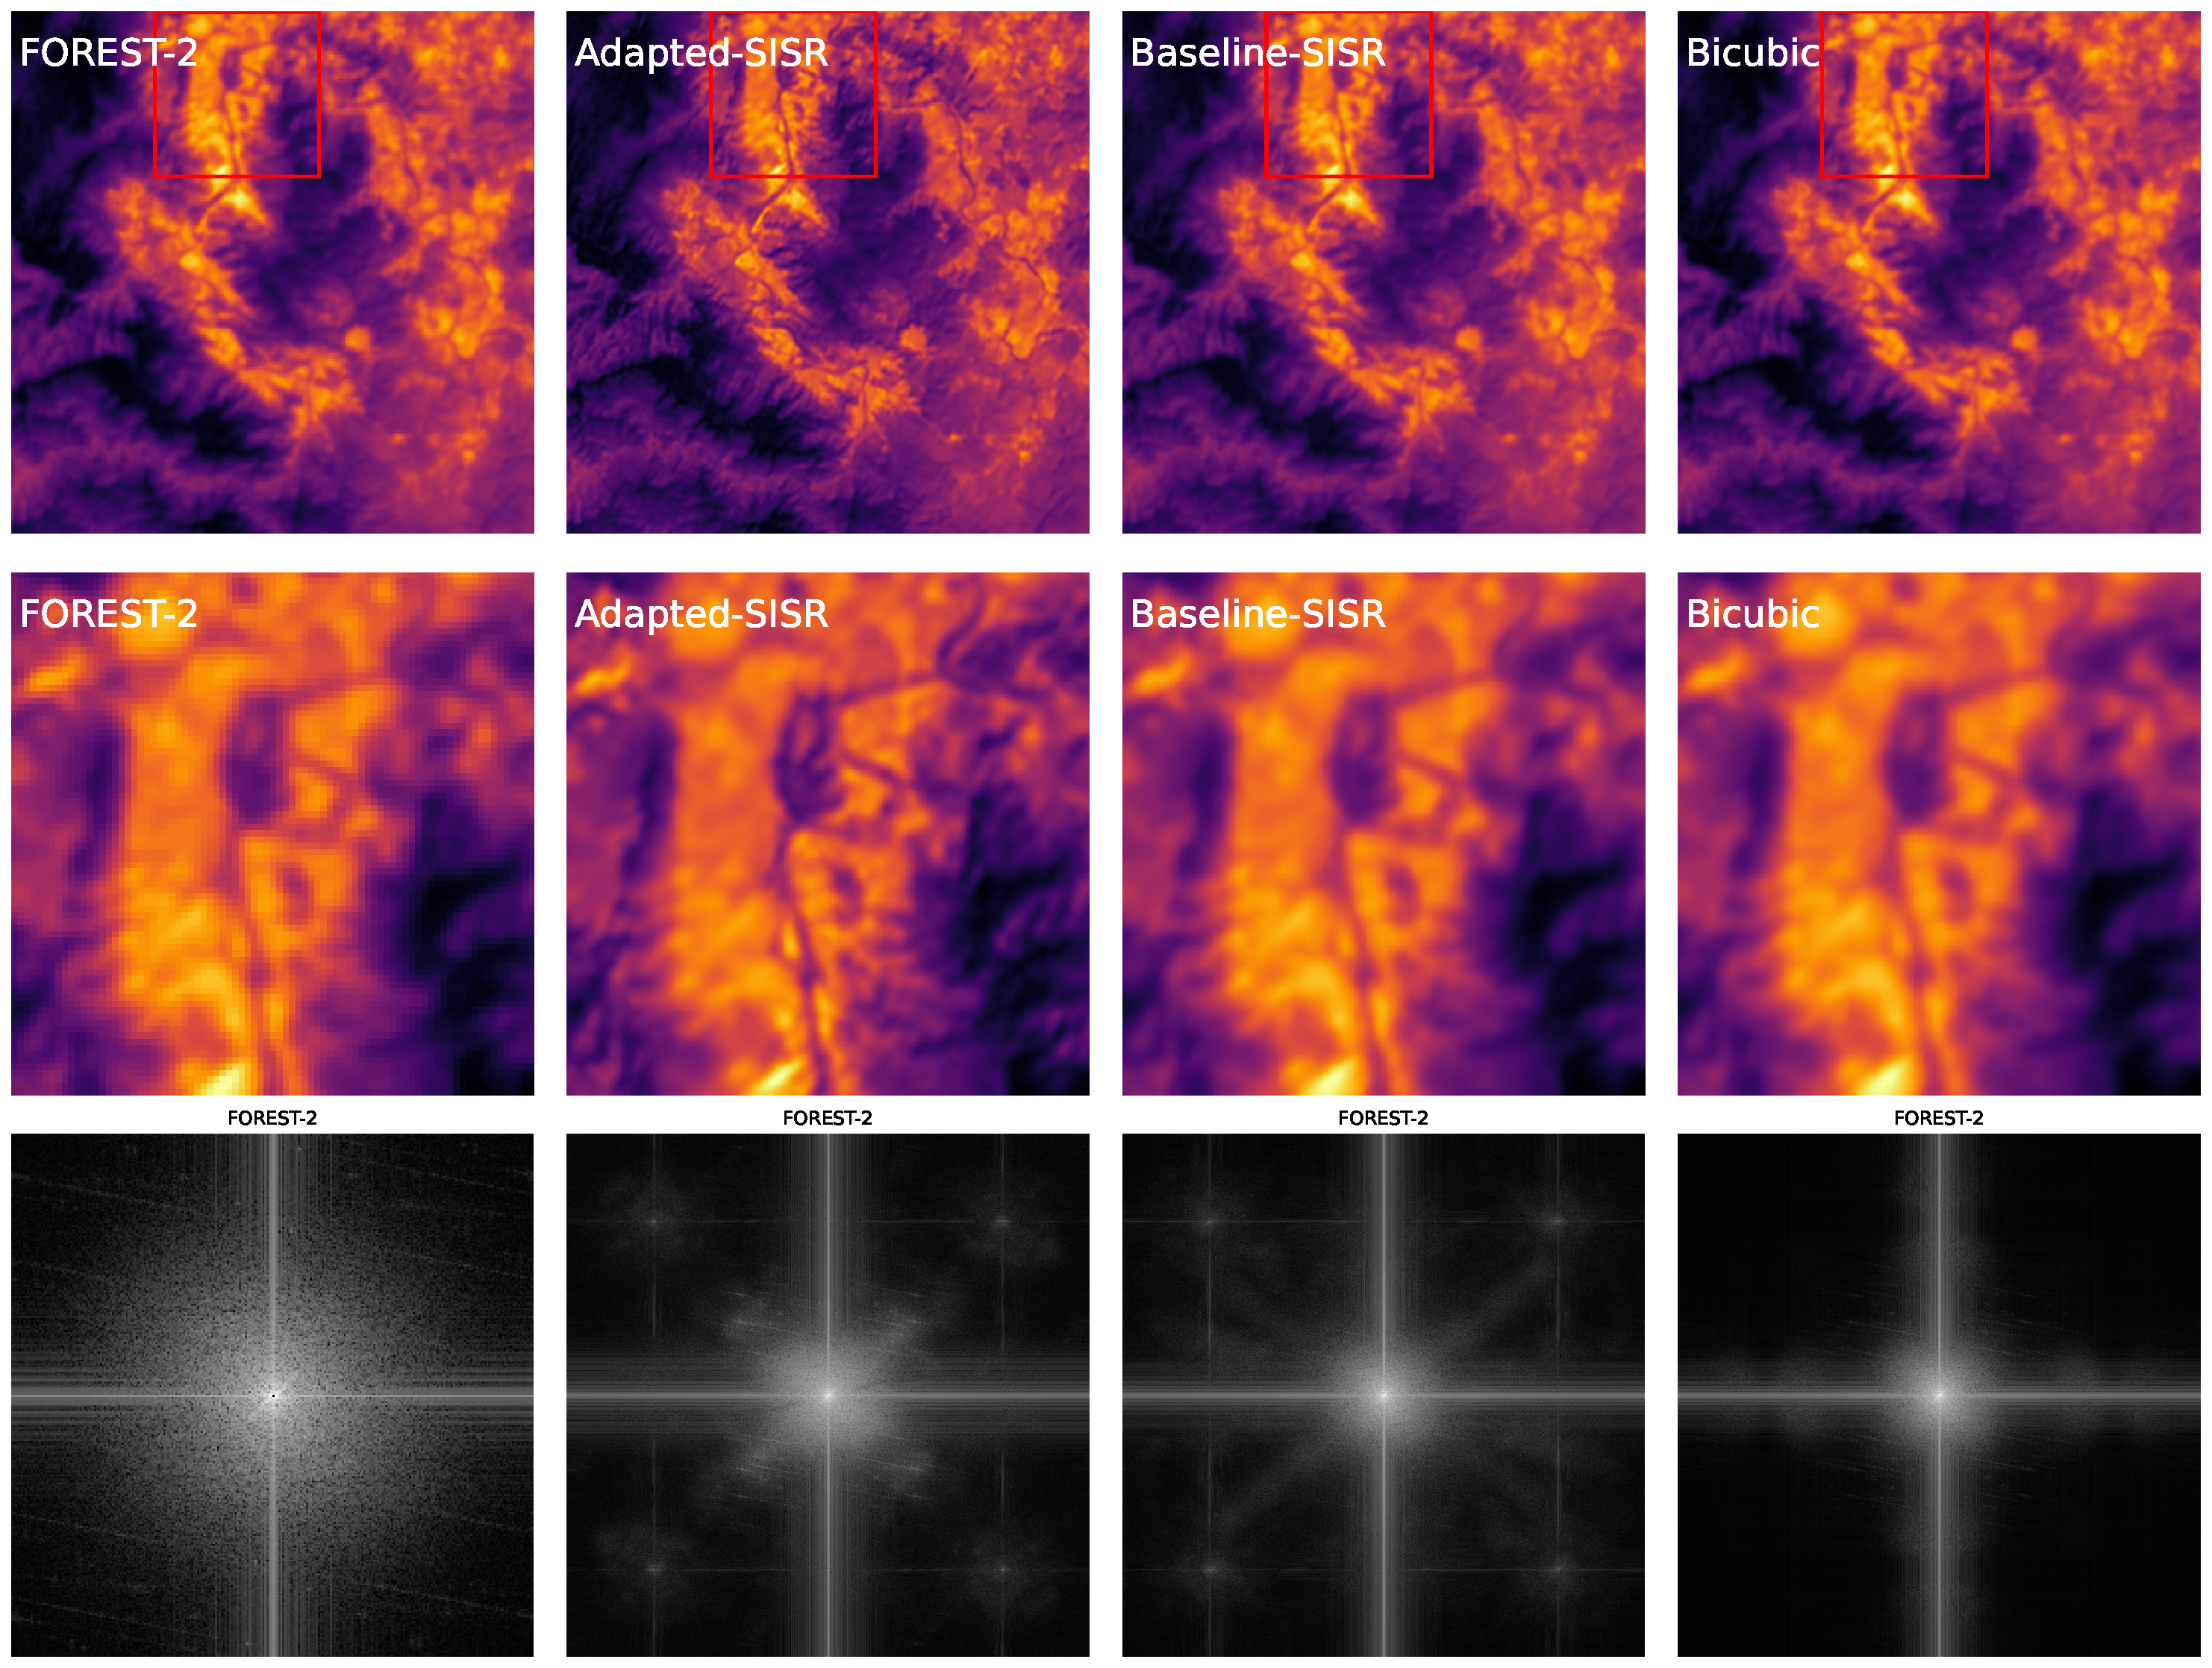
\includegraphics[scale=0.28]{Includes/5-target_prediction_sample.pdf}
            \caption{Super Resolved Forest-2 Scene using different SR models.
                     In the upper row, the image is displayed. A detailed zoom is displayed below. The original image is displayed in the left, while the super resolved images are displayed afterwards.
                    }
            \label{fig:5-target_prediction_sample}
        \end{figure}

        Fig. \ref{fig:5-target-amplification-statistics} shows a more detailed analysis of the frequency domain of the SR images obtained for the whole real FOREST-2 validation dataset.
        The effects of super resolution are clear, frequency components of interest are amplified in comparison to bicubic upsampling, without over-amplifying higher frequencies usually related to noise.  In (a),the log magnitude of the FFT for the SR images is displayed, adding a shade that represents the interval of ±1 standard deviations. 
        Up until 0.3 cycles per pixel, the adapted model has a higher log magnitude than the baseline SR model or bicubic upsampling, also staying slightly higher in high frequency components.
        As higher frequencies are related to noise and artifacts, this suggests that the adapted model is able to recover more details than the baseline model, while minimizing undesired components.
        The amplification plot of the SR models against bicubic upsampling shows the same behaviour in a more clear way. 
        The adapted amplification increases from the start of the plot and peaks between 0.08 and 0.25 cycles per pixel in a range of between 6 and 8 dB, on average, while the baseline model amplification lies between 0 and 2 dB.
        Such amplification, at a pixel size of 70m, corresponds to cycle frequencies between  300 $\frac{1}{m}$ and 875 $\frac{1}{m}$, which is consistent with the lost frequency components observed in \ref{fig:5-lr-images-fft-comparison}.
        
        On the other side, while the amplification is very similar in frequencies related to noise, the adapted model seems to step up a little bit compared to the baseline.  
        This suggests that the adapted model is able to recover details from real FOREST-2 images, amplifying frequencies of interest, at the cost of a small increase in the overall noise of the image.

        \begin{figure}[H]
            \centering
            \includegraphics[scale=0.5]{Includes/5-target-amplification-statistics.pdf}
            \caption{Frequency domain analysis of the SR images obtained by applying different SR models to the real FOREST-2 validation dataset.
            In (a), the log of the magnitude of the FFT for the SR images is shown,
            while in (b) the amplification with respect to a  simple bicubic upsampling is displayed.}
            \label{fig:5-target-amplification-statistics}
        \end{figure}


        In Fig. \ref{fig:6-target-gradient-analysis-image}, an example of the gradient analysis of the SR images is shown. 
        Compared to the baseline SISR model, the adapted model shows higher gradient magnitudes, suggesting that the adapted model is able to recover more details than the baseline model. 
        However, in the darker sections of the gradient magnitude, some small background noise can be observed, consistent with slightly increased amplification in the higher components of the frequency domain analysis from Fig. \ref{fig:5-target-amplification-statistics}.

        \begin{figure}[H]
            \centering
            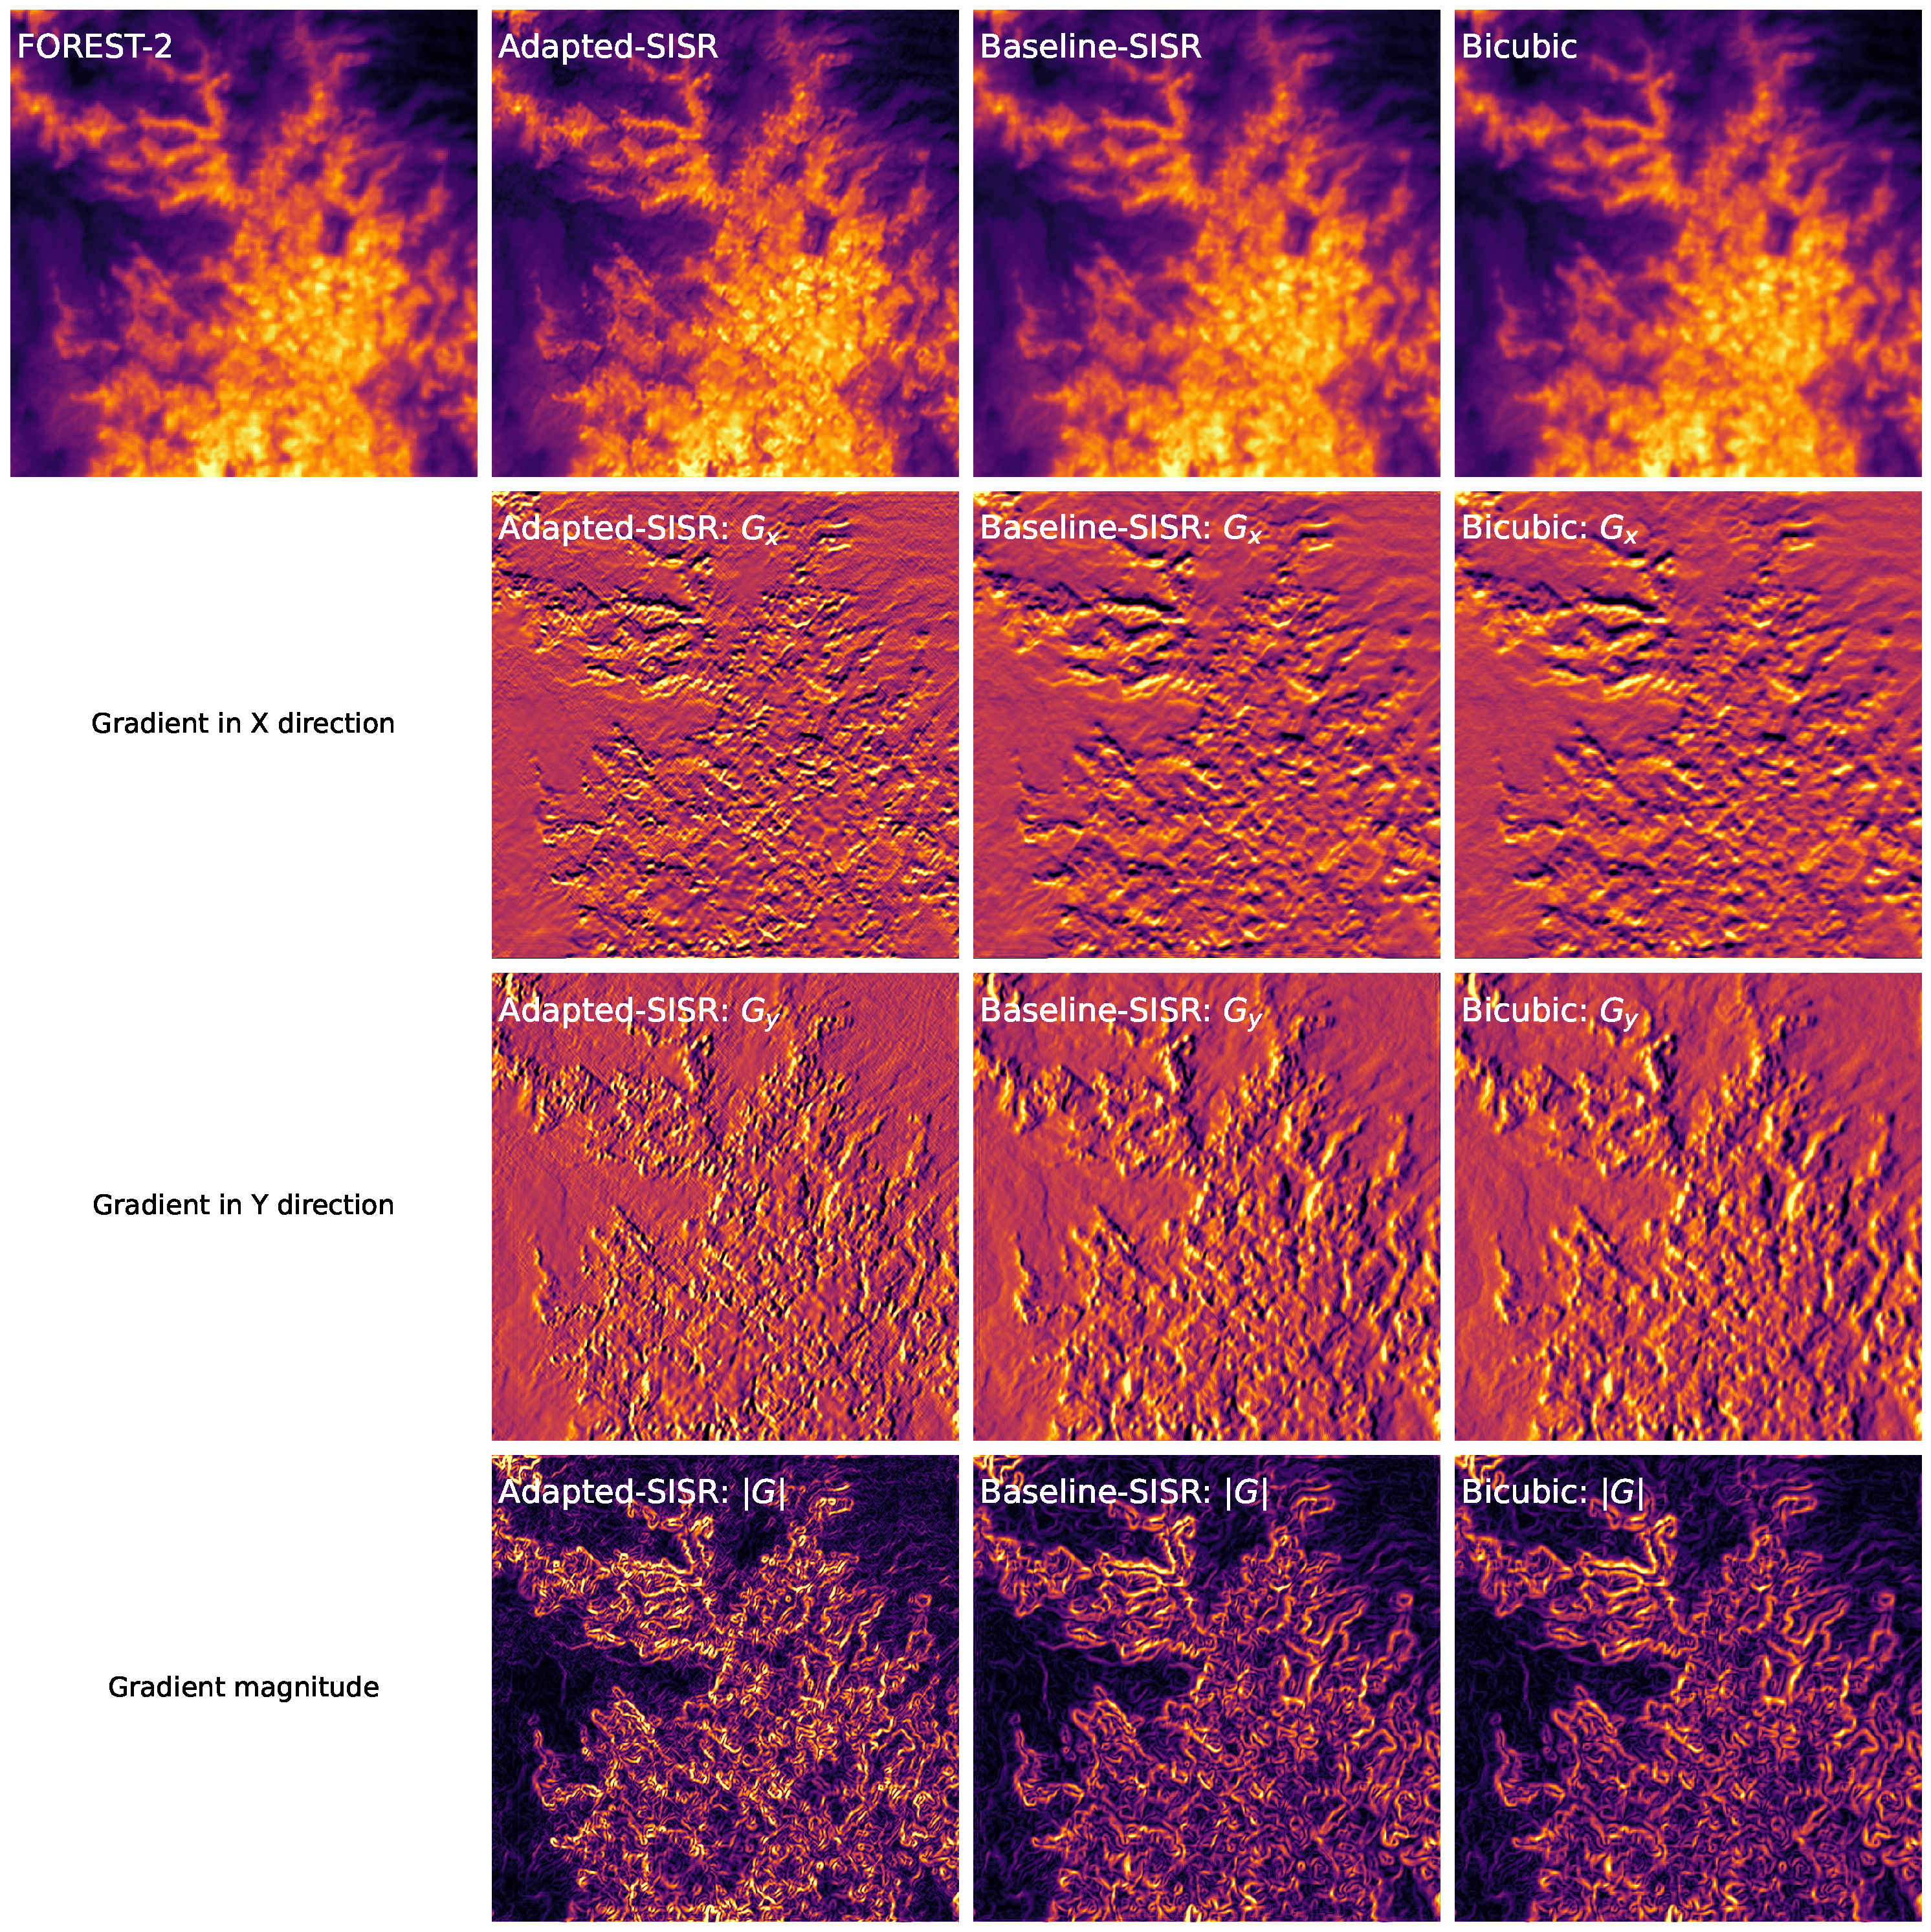
\includegraphics[scale=0.28]{Includes/6-target-gradient-analysis-image.pdf}
            \caption{Gradient analysis of the super resolved images using different SR models for scenes coming from the real FOREST-2 validation dataset.
                     In the upper row, the image is displayed. The gradients in the x and y direction ($G_x$ and $G_y$ respectiely) are displayed below.
                     the gradient magnitude $|G|$ is displayed in the bottom row.}
            \label{fig:6-target-gradient-analysis-image}
        \end{figure}

        Fig \ref{fig:5-gradient-histogram-validation-dataset} shows the estimated distribution function of the log gradient magnitudes of the whole validation dataset.
        Both the adapted and the baseline model show a decrease in the number of pixels with low gradient magnitudes compared to bicubic upsampling, suggesting that both models are able to recover more details.
        However, the adapted SR tends to have a higher high gradient magnitude pixels, implying that the adapted model is able to produce sharper edges than the baseline model.
        This is consistent with the observed results and the frequency domain analysis.
        % However, it is important to note that the gradient magnitude is not a good measure of the performance of the SR model, as it does not take into account the noise and artifacts that may be present in the image.
        % It represents only a complementary way to understand the effects of the SR model.

        \begin{figure}[H]
            \centering
            \includegraphics[scale=0.4]{Includes/5-gradient-histogram-validation-dataset.pdf}
            \caption{Density estimation of the gradient magnitude $|G|$ for the super resolved real FOREST-2 images from the validation dataset. The magnitudes of the Synthetic HR FOREST-2 images are also computed for comparison.}
            \label{fig:5-gradient-histogram-validation-dataset}
        \end{figure}

        In Fig. \ref{fig:5-correlation-histogram-validation-dataset}, the estimated density of the correlation coefficient between the pixels of an image and their neighbors is displayed for the whole validation dataset. 
        
        As expected for an image, the correlation is extremely high and the density is highly concentrated. The baseline and bicubic upsampling models have a very similar distribution, with the baseline SR being slighly skewed to the left.
        The adapted model has a broader distribution, less dense when closer to 1, implying that the pixels tend to be less correlated with their neighborhood. 
        
        \begin{figure}[H]
            \centering
            \includegraphics[scale=0.35]{Includes/5-correlation-histogram-validation-dataset.pdf}
            \caption{Density estimation of the correlation coefficient between the pixels and their neighborhoods, for the super resolved real FOREST-2 images from the validation dataset. The coefficients of the synthetic HR FOREST-2 images are also computed for comparison.}
            \label{fig:5-correlation-histogram-validation-dataset}
        \end{figure}

    \subsection{Sensibility to domain gap}

         % Another example would be images taken from FOREST-2 in several years may not have the same distribution as current images, as the instruments may have degraded over time.

        % To simulate this situation, the model trained using real FOREST-2 images was employed to super-resolve synthetic FOREST images degraded using the baseline degradation model. The results, shown in Figs. \ref{fig:5-target-prediction-with-domain-gap} and \ref{fig:5-target-prediction-with-domain-gap-fft}, indicate the performance of the adapted model is catastrophic, producing several artifacts and yielding a PSNR difference of approximately 10dB, which represents a tenfold difference in terms of Mean Squared Error (MSE). This highlights the critical need for adaptable SR models that can effectively handle diverse and evolving real-world scenarios.


        The combination of the probabilistic degradation model and the SR model were proven helpful to bridge the domain gap and improve the resolution of real FOREST-2 images.
        However, it is important to understand what happens when an arbitrary LR input that is not aligned with the target domain used in training is used.
        While the common scenario is that the real degradation model is more complex than the one assumed in the dataset generation, the opposite can also occur.
        As seen in \ref{subsec:results-lr-comparison}, assuming a more complex degradation model in the dataset could lead to LR inputs with more attenuation in critical frequency components, resulting in an SR model that "over-amplifies" to generate an HR output, leading to noisy images with undesired artifacts.
        In this particular experiments, HR-LR pairs generated using the baseline degradation model exemplify an overly optimistic degradation scenario and will be used on the SR models of each pipeline.
        As in this experiment the ground truth is known, the performance of the SR model can be evaluated using metrics like PSNR and SSIM. Additionally, a frequency domain analysis with respect to the ground truth can be done.
        
        The results are shown in Figs. \ref{fig:5-target-prediction-with-domain-gap} and \ref{fig:5-target-prediction-with-domain-gap-fft}.
        The performance of the adapted model on LR images coming from the baseline degradation model is catastrophic, producing several artifacts and yielding a PSNR difference of approximately 10dB, which represent a 10x difference in terms of MSE.

        \begin{figure}[H]
            \centering
            \includegraphics[scale=0.28]{Includes/5-target_prediction_sample-with-domain-gap.pdf}
            \caption{Effects of using a model trained  on a different domain than at inference time. 
                     When using an Synthetic FOREST image degraded with the baseline degradation model as an input, the model trained using real FOREST-2 data as the target domain generates several artifacts and underperforms severely in terms of PSNR. }
            \label{fig:5-target-prediction-with-domain-gap}
        \end{figure}

        The frequency domain analysis of the ground truth and the super resolved images are shown in Fig. \ref{fig:5-target-prediction-with-domain-gap-fft}.  
        The adapted model amplifies frequencies with respect to the ground truth, something that should not happen in any SR task. 
        This suggests that while the adapted model may highlight edges and details, it also severely amplifies the noise and artifacts, resulting in a worse performance in terms of PSNR.
        

        \begin{figure}[H]
            \centering
            \includegraphics[scale=0.4]{Includes/5-target-prediction-with-domain-gap-fft.pdf}
            \caption{Effects of using a model trained with on different domain than at inference time. 
                     (a) shows the log magnitude of the radial average of the FFT for the SR images using different algorithms.
                     (b) shows the amplification with respect to bicubic interpolation.
                     }
            \label{fig:5-target-prediction-with-domain-gap-fft}
        \end{figure}

        Fig \ref{fig:5-target-amplification-statistics-with-domain-gap} shows the results of the frequency domain analysis for the whole validation dataset. The results seem to be consistent in the range observed in Fig. \ref{fig:5-target-prediction-with-domain-gap-fft}. Having frequency amplification with respect to the ground truth is a display of the inability of the adapted SR model to reconstruct the ground truth image properly.
        
        The adapted model was trained on generated LR images that try to mimic the real FOREST-2 images, which have a more complex degradation model. This results in an SR model that tries to reconstruct the ground truth from a "blurrier" starting point, learning to amplify some frequencies much more than what is needed when the LR images come from the baseline degradation model.


        \begin{figure}[H]
            \centering
            \includegraphics[scale=0.4]{Includes/5-target-amplification-statistics-with-domain-gap.pdf}
            \caption{Effects of using a model trained with on different domain than at inference time, statistics over the whole validation dataset. 
                     (a) shows the log magnitude of the radial average of the FFT for the SR images using different algorithms.
                     (b) shows the amplification with respect to bicubic interpolation.
                     Painted areas represent ±1 standard deviations.
                     }
            \label{fig:5-target-amplification-statistics-with-domain-gap}
        \end{figure}

        The performance results in terms of different metrics are shown in Fig. \ref{fig:5-target-prediction-with-domain-gap-dataset}. 
        In the conditions described above, the adapted super resolution model underperforms severly in every considered metric.


        \begin{figure}[H]
            \centering
            \includegraphics[scale=0.38]{Includes/5-target-prediction-with-domain-gap-dataset.pdf}
            \caption{Performance obtained by super resolving the degraded synthetic FOREST images using different super resolution models. The Pearson correlation coefficient is represented by $\rho$.}
            \label{fig:5-target-prediction-with-domain-gap-dataset}
        \end{figure}
        
        
    This demonstrates that while this approach is very good to bridge a domain gap, it is not robust at all to domain shifts. 
    This limitation is in sync with what is found in the literature seen in \ref{subsubsec:implicit-modelling}. Implicit modelling for blind super resolution using GANs are not able to generalize to arbitrary domains not seen in the target domain.

    \subsection{Domain gap assessment using non-referenced image quality assessment}

    As in the target domain the ground truth is not known due to the lack of a paired dataset, the performance of the SR model can not be evaluated using metrics like PSNR and SSIM.
    Non-referenced image quality assessment (NR-IQA) metrics can help to understand the relative performance of the SR models when arbitrary LR images are used as an input.
    
    The analysis was performed by taking the adapted and baseline SR models and using them to super resolve LR images coming from the baseline degradation and real LR forest-2 images as an input.
    Then, the NIQE and BRISQUE scores are calculated.
    
    The results are shown in Fig. \ref{fig:5-target-iqa-results}.
    For both metrics, a large gap is observed between the adapted model and the rest when the input is real FOREST-2 data.
    This behaviour does not replicates when the input LR images are generated using the baseline degradation. Moreover, for the adapted model, both metrics tend to get worse when the input images are not real FOREST-2 images. The contrary happens for the rest of the models.

    \begin{figure}[H]
        \centering
        \includegraphics[scale=0.25]{Includes/5-target-iqa-results.pdf}
        \caption{Image quality assessment metrics for the different SR models using different datasets as input. }
        \label{fig:5-target-iqa-results}
    \end{figure}

    
    This suggests that the SR model is able to produce more natural images only when the input images come from the same distribution as the target domain used in training. However, it is important to note that: 

    


    \begin{enumerate}
        \item NIQE and BRISQUE are calculated using a pre-trained model. The images used for the pre-training are not remote sensing images, and therefore, the results may not be representative. This could be circumvented by training a NIQE/BRISQUE model trained with a more adequate dataset for the task.
        \item NIQE and BRISQUE are a measure of image quality and naturalness, not physical consistency or reconstruction fidelity.
    \end{enumerate}
        
\newpage
    
\section{Conclusions}

In this work, the feasibility of applying blind single-image super resolution algorithms to thermal remote sensing data from OroraTech’s FOREST-2 mission was studied. The study is centered on the following research questions:

\begin{itemize}
    \item What is the impact of the unknown FOREST-2 degradation model compared to the one commonly used for dataset generation?
    \item Is it possible to estimate the FOREST-2 degradation model using a data-driven approach?
    \item How can the degradation model be incorporated into training to improve SR results?
    \item  How can the SR results be assessed when paired data is scarce?
\end{itemize}

To have HR data, an automated process was developed for fetching, filtering, and processing data from third-party, higher-resolution missions. The conventional method for dataset pair generation of bicubic downsampling + white noise was proven inadequate in section \ref{sec:results}. The domain gap between the artificially degraded and real LR images was shown to be too wide, resulting in an SR model that is not able to generalize to FOREST-2 images and renders blurry results.

Blind super resolution techniques were explored as a solution in section \ref{sec:methodology}. The current lack of paired ECOSTRESS and FOREST-2 data leads to the use of implicit modeling for the data-driven degradation process estimation through a GAN architecture. A probabilistic degradation model was proposed for the task, mainly for three reasons. First, its well-constrained kernel and noise modules allow the training of an end-to-end pipeline of degradation and SR. Second, using deep learning to generate the kernel and noise facilitates the analysis of the degradation process and comprehension of its effects. Third, the stochastic nature of the proposed architecture allows sampling from the degradation distribution to generate a wide variety of HR-LR pairs from only one HR image, which is very useful for augmenting training datasets.

The degradation model adapted to FOREST-2 images and its effects were studied by comparing them to a baseline degradation in section \ref{sec:results}. The results showed that the adapted degradation model produces LR images that are consistently blurrier and have powerful noise that is usually strongly correlated with the content of the image. Although stronger degradation was introduced, the SR results for both pipelines are similar. 
% Thus, the SR model, despite starting from different LR images, can reconstruct the original image with comparable quality. 
This display of capacity suggests that the SR model is probably being under-utilized when using baseline degradations. However, an upper bound to the PSNR is observed, regardless of the LR input. The introduction of newer SISR methods or multi-spectral SR may be beneficial to overcome this limitation in reconstruction performance.

When comparing the results of the adapted SR model with the baseline on real FOREST-2 images, more detail and edges seem to be present at the cost of a small increment in the overall noise. The implemented framework of unpaired image comparison consisting of frequency domain, gradient and pixel-neighborhood correlation analysis also yielded positive outcomes. 
The images have more power in a wide range of frequencies when compared to bicubic upsampling, in the order of 6dB. The amplified frequencies match the ones lost during the degradation process, implying that the adapted SR model is able to recover part of the signal. The observations from the gradient magnitude and pixel-neighborhood correlation analysis corroborate the results. Moreover, the model was also tested in a single paired scene from ECOSTRESS and FOREST-2, revealing it has higher performance and can highlight subtle features such as small islands that were almost undetectable using traditional upsampling methods. Nevertheless, the limited number of available images does not allow for drawing definitive conclusions.

The sensitivity to differences between training data and arbitrary inputs is a very relevant result, as it shows the limitations of the implicit modeling approaches. While they help to bridge the domain gap, they are not able to generalize to an arbitrary input that is outside of the target domain.
When applying the adapted SR model to bicubic downsampled images, the resulting image quality proved to be unusable.
In this case, the direction of the gap is inverted. The estimated degradation kernel is more complex than the actual one, resulting in SR over-amplifying frequencies. This also highlights the difficulty of hand-picking the degradation model in classical dataset generation techniques, as it is easy to be overly optimistic or pessimistic when choosing the amount of degradation.
The sensitivity to domain shifts was also analyzed using non-referenced image quality assessment metrics, where the domain-adapted SR model had a significantly better score only when the input was real FOREST-2 images. 

Overall, the combination of probabilistic degradation modeling and SR yielded promising results. It is a flexible approach in the sense that it only requires two sufficiently large datasets that do not need to be paired. 
The drawbacks of implicit modeling are not as relevant in this application compared to other tasks because the conditions of the missions (and their degradation models) are almost static. Unlike other applications such as smartphone images, where the number of possible cameras and sensors is practically infinite, the number of sensors in a satellite remains the same, and only the change of conditions due to the passing of time should be considered. This means that the degradation model can be trained on a particular domain, and the LR input that will be used in the future will probably come from the same distribution. The end-to-end nature of this training framework allows to have multiple SR models, one for each wanted target domain, with low difficulty.

% The implemented framework leverages implicit modeling to estimate a degradation model and produce LR images that can be analyzed to study its impact on the SR process. This information is also incorporated into the training process to produce better results.
% The development of methods for assessing SR performance without paired HR-LR images is also an important contribution due to the scarce nature of this type of data. While they may not be sufficient to quantify the performance of the SR model, they are a good indicator of the quality of the results.

\subsection{Future Work}

This work has laid the groundwork for doing degradation-aware super resolution of FOREST-2 images without the need for paired data. While the results are promising, several assumptions can be challenged, and many avenues remain unexplored. The following points outline promising directions for future research:

\begin{itemize}

    \item The HR dataset obtained from ECOSTRESS is based on the similarities in the spectral domain between the two missions. While their characteristics are very similar, they are not the same, and the implications of this mismatch should be further studied.
    
    \item Despite using unpaired data for training, the lack of a paired HR-LR dataset still poses a challenge. One single scene does not allow for drawing definitive conclusions on the performance of the model. Moreover, the availability of a paired dataset composed of more images would allow for better training decisions, leveraging techniques like early stopping for model selection. 
    
    \item The probabilistic degradation modeling assumes independence between the noise and kernel components. While it is a reasonable assumption, it may not hold in all cases.
    
    \item The addition of a discriminator that distinguishes between the HR image and the super-resolved  LR images coming from the target domain may improve the quality of the results even further. It may do so by aligning their distributions without the need for them to be paired.
    
    \item Due to the sensibility to any domain shift, investigating pre-processing methods for detecting inputs that are out-of-distribution with respect to the training data before using the SR models may prove helpful in avoiding undesirable results.
    
    \item The introduction of novel SISR architectures, or the incorporation of information from other spectral bands to use MSSR as in \cite{myself2023}, may be beneficial to overcome the limitations of the SR model. If multi-image data from FOREST-2 is available, MISR is also a very promising alternative.
    
    \item In the future, OroraTech will launch a constellation of cubesats that will have identical hardware. Still, the degradation model may be slightly different due to manufacturing tolerances and performance degradation over time. When more data is available, it will be necessary to investigate whether a general model for all FOREST data products is possible or if each cubesat needs its own model.
    
    \item While the NIQE and BRISQUE metrics help assess the quality of SR without a reference, their corresponding models are trained on natural images. The development of NIQE and BRISQUE metrics trained on remote sensing data may be more suitable for the task.
    \item Because of how the frequency domain analysis is done, the value of a particular spatial frequency is the average over every direction. This approach could be further developed to focus on specific directions.
    
\end{itemize}


\newpage

\pagestyle{empty}
\bibliographystyle{unsrt}
\bibliography{bibliography}



\end{document}


